              
                %% bare_jrnl.tex
%% V1.4b
%% 2015/08/26
%% by Michael Shell
%% see http://www.michaelshell.org/
%% for current contact information.
%%
%% This is a skeleton file demonstrating the use of IEEEtran.cls
%% (requires IEEEtran.cls version 1.8b or later) with an IEEE
%% journal paper.
%%
%% Support sites:
%% http://www.michaelshell.org/tex/ieeetran/
%% http://www.ctan.org/pkg/ieeetran
%% and
%% http://www.ieee.org/

%%*************************************************************************
%% Legal Notice:
%% This code is offered as-is without any warranty either expressed or
%% implied; without even the implied warranty of MERCHANTABILITY or
%% FITNESS FOR A PARTICULAR PURPOSE! 
%% User assumes all risk.
%% In no event shall the IEEE or any contributor to this code be liable for
%% any damages or losses, including, but not limited to, incidental,
%% consequential, or any other damages, resulting from the use or misuse
%% of any information contained here.
%%
%% All comments are the opinions of their respective authors and are not
%% necessarily endorsed by the IEEE.
%%
%% This work is distributed under the LaTeX Project Public License (LPPL)
%% ( http://www.latex-project.org/ ) version 1.3, and may be freely used,
%% distributed and modified. A copy of the LPPL, version 1.3, is included
%% in the base LaTeX documentation of all distributions of LaTeX released
%% 2003/12/01 or later.
%% Retain all contribution notices and credits.
%% ** Modified files should be clearly indicated as such, including  **
%% ** renaming them and changing author support contact information. **
%%*************************************************************************


% *** Authors should verify (and, if needed, correct) their LaTeX system  ***
% *** with the testflow diagnostic prior to trusting their LaTeX platform ***
% *** with production work. The IEEE's font choices and paper sizes can   ***
% *** trigger bugs that do not appear when using other class files.       ***                          ***
% The testflow support page is at:
% http://www.michaelshell.org/tex/testflow/


% Please refer to your journal's instructions for other
% options that should be set.
%\documentclass[journal,twocolumn]{IEEEtran}
\documentclass[12pt, draftcls, onecolumn]{IEEEtran}



\usepackage{soul,xcolor}
\usepackage{bm}
\include{graphics}
\include{amsmath}
\usepackage[normalem]{ulem}
\usepackage{multirow,enumitem}
\usepackage{algorithm}
\usepackage{algpseudocode}
\usepackage{verbatim}
\usepackage[latin1]{inputenc}
\usepackage{amsmath}
\usepackage{amsfonts}
\usepackage{amssymb}
\usepackage{mathrsfs}
\usepackage{booktabs}
\usepackage{url}
\usepackage[pdftex]{graphicx}
% \usepackage[skip=1pt,font=scriptsize]{subcaption}
\usepackage{ifthen}
\usepackage{xspace}
\usepackage{dsfont}
\usepackage{bbm}
\usepackage{cite}
\usepackage{epsfig}
\usepackage{epstopdf}
\usepackage{array}
\usepackage{multicol}
\usepackage{algpseudocode}
\usepackage{algorithm}
\usepackage{breqn}
\usepackage{esint}
% \usepackage[skip=2pt,font=footnotesize]{caption}
\usepackage{multicol}
\usepackage{amsthm}
\usepackage{setspace}
\usepackage{lipsum}
% \usepackage{dblfloatfix}
% \hyphenation{op-tical net-works semi-conduc-tor}
\renewcommand\qedsymbol{$\blacksquare$}
\theoremstyle{plain}
\newtheorem{theorem}{Theorem}
\newtheorem{lemma}{Lemma}
\theoremstyle{definition}
\newtheorem{corollary}{Corollary}
\newtheorem{remark}{Remark}
\theoremstyle{remark}
\newtheorem{nota}{Notation}
\usepackage{footnote}

\newcommand{\nt}[1]{\textcolor{red}{\textbf{[#1]}}}
\newcommand{\tc}[1]{\textcolor{magenta}{\textbf{[TC: #1]}}}
\newcommand\norm[1]{\left\lVert#1\right\rVert}
\newcommand{\round}[1]{\ensuremath{\left\lfloor#1\right\rceil}}
\usepackage{bbold}
\usepackage{todonotes}
\newtheorem{definition}{Definition}
\usepackage{stmaryrd}
\usepackage{algorithm,algcompatible}
\algnewcommand\INPUT{\item[\textbf{Input:}]}%
\algnewcommand\OUTPUT{\item[\textbf{Output:}]}%
% \usepackage{cite}
\usepackage{lipsum}
\usepackage{mathtools}
\usepackage{cuted}
\usepackage{stfloats}% <-- added
% *** GRAPHICS RELATED PACKAGES ***
%
\ifCLASSINFOpdf

\else

\fi







\begin{document}

% \title{Bare Demo of IEEEtran.cls\\ for IEEE Journals}


\title{Millimeter Wave Channel Learning Aided by Tensor Completion}
\author{Tzu-Hsuan~{Chou}, Nicolo {Michelusi}, David J. {Love}, and James V. {Krogmeier}
% \nm{coauthors?}
\thanks{The authors are with the School of Electrical and Computer Engineering, Purdue University, West Lafayette, IN, USA; emails: \{chou59, michelus, djlove, jvk\}@purdue.edu.}% 
\thanks{This research has been funded by NSF under grant CNS-1642982.}
}


\maketitle

\begin{abstract}
\end{abstract}

\begin{IEEEkeywords}
Millimeter wave, beam-alignment, position-aided, tensor completion, sparse learning.
\end{IEEEkeywords}

\IEEEpeerreviewmaketitle

\section{Introduction}
% (1 paragraph) motivation. 
% massive MIMO and mmWave
% \nt{motivation} \nt{mmWave and massive MIMO are solutions}
%\nt{motivation}
Future wireless communication system needs to sustain the condition for higher data rates, lower latency, and better power efficiency \cite{6824752}.
In last few years, millimeter wave (mmWave) communication gains more attentions and be the promising candidate to provide the throughput enhancement for the future wireless network (5G) due to abundant available bandwidth in the spectrum \cite{6515173,7400949,6736761,6736746}.
The narrow beam property of mmWave is also beneficial for the network quality with the interference reduction.
However, the mmWave communication experiences higher path loss than conventional sub-6GHz system, led by air, water, and vapor absorption resulting in the link quality degradation.
To conquer the adverse channel condition and to utilize the narrow beam property, it demands the great beamforming gain from the fast and high directional transmission. 

%\nt{introduce massive MIMO}
The wavelength of mmWave is relatively small that allows the devices packing large number of antennas in small-scale area, especially suitable for Massive MIMO system.
% The spatial sparsity of mmWave propagation with few dominant clusters (paths) drives a set of beam-alignment scheme on directional transmission.
The conventional MIMO system using the same number of RF chain as the number of antennas, called digital (baseband) beamforming, may be unsuitable to be applied in massive MIMO system due to the high cost and power consumption of RF chains.
To conquer the disadvantage, the analog beamforming with one RF chain is considered in several works\cite{6600706,6979962}.
Analog beamforming ususally uses the phase shifter with constant modulous constraint, such as uniform linear array (ULA) and uniform planar array (UPA).
ULA is the phase shifted multiple antennas vector.
The system with ULA has been widely studied in \nt{ref}.
UPA \cite{6525612,7947209} is the array vector packed with the antennas in planar grid, utilizing the 3D beamforming pointing in certain direction with the elevation angle and azimuth angle to provide the beamforming gain, and to eliminate the inter-user interference.
\nt{Hybrid precoding, TBD}

% These beam-alignment scheme ranges from beam-sweeping \cite{8573158}, AOA/AOD estimation \cite{6847111,7390019}, to data-assisted scheme \cite{7952807,Va2018, 8445969}.

% (2 paragraph) challenges must be addressed. 
% \nt{address the challenges}
%\nt{challenges: beam-alignment technique, and review prior work on these challenges}
The traditional channel acquisition in massive MIMO system is unworkable because of the great number of antennas which induce the unacceptibly high channel estimation overhead.
It is pessimistic for the massive MIMO because the enormous channel estimation (training) overhead occupies most of the channel coherence time, leading to inadequate amount of time for transmission even it has large gain margin from accurate beamforming.
Therefore, the fast and accurate beam-alignment protocol is demanding for enabling the massive MIMO in mmWave communication.
The spatial sparsity of mmWave propagation with few dominant clusters (paths) drives a set of beam-alignment scheme on directional transmission.
% (2 paragraph) what others have done wrt challenges listed in the 2nd bullet. Do a thorough review .
% \nt{What other reference have done wrt challenges listed above.}
% \nt{Review prior work of beam-alignment, TBD} 
To facilitate the mmWave communication system, the beam-alignment schemes, ranging from beam-sweeping \cite{8573158}, AOA/AOD estimation \cite{6847111,7390019}, to data-assisted scheme \cite{7952807,Va2018, 8445969}, are intensely investigated in recent years.
Beam-sweeping requires collecting a set of measurements of the possible beam-directions.
The exhaustive search is the simplest way belonging to this group, which check the performance of all possible beams.
AOA/AOD estimation leverage the spatial sparsity of mmWave channel via compressive sensing technique. \nt{introduce previous works.}
Regarding the data-assisted scheme, it employs the side information to capture and provide the relation with mmWave channel.
The mmWave channel are related to the situation of user, like the user's position, the geometry of environment, the traffic condition, or the accessed base station.
\nt{introduce previous works.}
% In \cite{Va2018,8445969}, they develop the beam recommendation algorithm for the user's positions where the prior measurements are available. 
In \cite{Va2018}, it considers the mmWave beam alignment in V2I system with multipath fingerprint which utilizes the long-term channel characteristics associated with the position.
In \cite{8445969}, it does the beam recommendation by extracting the information from the prior measurement with the help of position information and environmental situational awareness.
It is worth noting that the previous position-aided method develop the beam recommendation algorithm only for the user's positions where the prior measurements are available.


%\nt{Review prior work of matrix/tensor completion, TBD.} 
%Matrix/tensor completion supports estimating the missing values of the data in matrix/tensor with the available information and the properties of the data structure.
%The real-world data normally exhibits correlations between elements, like continuity, symmetry, smoothness, low-rankness, etc.
%Several completions techniques are widely utilized in computer vision, image in-painting, recommendation systems.
%The two most popular properties applying for completion are the smoothness \cite{Rudin:1992:NTV:142273.142312,XuHan2014} and low-rankness.
%In \cite{Rudin:1992:NTV:142273.142312}, the total variation (TV) is applied as a smoothness constraint for image completion.
%In \cite{XuHan2014}, a modified linear total variation was proposed as a smoothness constraint and exploited with the low-rank matrix completion (LTVNN).
%
%\nt{Review prior work of channel charting, TBD}
%Channel charting\cite{8444621} is the novel framework in MIMO network, learning the chart of radio geometry in the service area.
%The core idea of channel charting is that the users close in spatial position would experience similar CSI.
%In \cite{8444621}, the channel charting is used to locate users in service area without acquiring precise location information from global positioning systems (GPS).
%The radio geography is charted based on the statistical CSI, which is essential for extracting the information.
%%In \cite{8444621}, it focuses on the second order statistical moment of the received CSI.



%Channel charting is the technique which records the statistical CSI for
% (1 paragraph) how the papers in 3rd bullet do not solve all problems in the second bullet. 
% The problem not yet solved.
% \nt{What is the problem not yet solved in above introduction}
% All the previous beam-alignment method in data-assisted scheme requires the prior measurements in the user's position.
\nt{Problem not yet solved} In all previous beam-alignment method with data-assisted scheme, the database is expected to contain the prior measurements for the entire service area.
It requires costly measurement and huge overhead for the data collection, so the assumption of the prior work is inefficient.
Once the user is located in the position without prior measurement, the prior works fail to provide accurate recommended beam sets for user.


% (2 paragraph) Explain what to do and how it is different from papers in previous work. 
% Explain this paper.
% low-rank and smoothness

\nt{Idea of Channel Learning}\nt{Matrix completion/ Tensor Completion, TBD}


% \nt{Explain what to do. What's difference from previous work.}
% \nt{How do we provide the solution? low-rank + smoothness}
\nt{Explain my work, TBD}%\nt{Channel charting aided by Tensor Completion}
%In this paper, we propose a learning-based recommendation algorithm to mitigate the training overhead of the position-aided beam alignment protocol.


% In this work, we propose a channel recommendation algorithm to reduce the training overhead in the position-aided beam alignment protocol.
% To learn the function mapping between received power and side information (e.g. position and beam-pair), we model the database into the expression of tensor, where we consider the dimensions.



% Organization.
\nt{Organization:}

% Section 2
\section{System Model and Problems Formulation}
% Subsection 2.1
\subsection{General System Model}
% (2 paragraph) system model. 
We consider a scenario with a base station (BS), serving an area with GPS coordinates $\{(g_x,g_y):X_0\leq g_x\leq X_{end},Y_0\leq g_y \leq Y_{end}\}$, as in Fig. \ref{fig:wireless_comm_scenario}.
% 1 for MIMO channel
%We consider a uplink MIMO communication with a narrowband frequency-flat, block-fading channel between single base station (BS) and single mobile user (UE).
%The base station is equipped with $N_r$ receive antennas and the user has $N_t$ transmit antennas.
Considering a uplink MIMO scheme, in which the UE at GPS coordinate $\mathbf g=(g_x,g_y)$ sends an $N_t\times 1$ transmit signal vector $\mathbf x$, yielding the $N_r\times 1$ received signal vector 
%The MIMO system can be expressed as the form
\begin{equation}
    \mathbf{y}_{\mathbf g}=\mathbf{H}_{\mathbf g}\mathbf{x} + \mathbf{n}
\end{equation}
where $\mathbf{H}_{\mathbf g}$ is an $N_r\times N_t$ uplink channel matrix between the BS and the UE at GPS coordinate $\mathbf g$, and $\mathbf{n}$ is an $N_r$-dimensional noise.
Assume that the noise to have i.i.d. entries distributed as $\mathcal{CN}(0,\sigma_n^2)$.
Here, the channel is related to the position of BS, UE, and clusters in the environment.
To the best of our knowledge, this channel model can only be done by real channel measurements or the simulation by ray-tracing software, which simulates the channel measurements from the accurate modeling of the propagation environment.
%The ray-tracing channel simulation is considered to generate the MIMO channel.
%\nt{Explain ray-tracing/map-based channel.}
%The ray-tracing simulation generates the channel by providing AoA, AoD, and channel coefficients from the accurate modeling of the propagation environment.
%These channel information are based on BS's position, UE's position, and the clusters of the environment.
%In \cite{3gpp.38.901}, this method is named as map-based channel model.
In \cite{3gpp.38.901}, it studies and states the channel modeling of physical layer based on the propagation environment, called map-based channel model.
Our proposed algorithm is applicable to the channel acquired by real measurements, but we generate the channel measurement with the simulator, Quadriga \cite{6758357}, for the evaluation.
%We propose the algorithm applicable to the channel acquired by real measurements.
%We propose the algorithm applicable to the real channel measurements.
%For the aspect of evaluation, we generate the channel measurement with the simulatior, Quadriga \cite{6758357}.
In the work, the position of the BS and clusters are fixed , so the wireless channel should be strongly related to the UE position.
%In this work, we consider that the clusters are fixed in the environment, so the wireless channel depends only on the positions of the BS and the UE.
%Thus, the variation of channel is caused by the mobility of UE.


% 1 for the beamformer vector codebook





%For the use of the position information, we describe how we label the positions in service area. 
%The position information is available in mobile phone or automobile via a set of sensors, like GPS, camera, or LIDAR.
%Considering a scenario with one BS serving a area with GPS coordinate $\{(g_x,g_y):X_0\leq g_x\leq X_{end}, Y_0\leq g_y\leq Y_{end}\}$, we discretize the area by the separation distance $\Delta_s$ into $\mathbf{p}=(p_x,p_y)$ in the grid, expressed as
%$$(p_x,p_y)=\left(1 + \round{\frac{g_x-X_0}{\Delta_s}},1 + \round{\frac{g_y-Y_0}{\Delta_s}}\right),$$
%where $\round{x}$ means the nearest integer to $x$; the x-axis label $p_x\in \{1,\cdots,N_{p_x}\}$, where $N_{p_x} = \left\lceil\frac{X_{end}-X_0}{\Delta_s}\right\rceil$; and the y-axis label $p_y\in \{1,\cdots,N_{p_y}\}$, where $N_{p_y} =\left\lceil \frac{Y_{end}-Y_0}{\Delta_s}\right\rceil$.
%% Intuitively, the channels are related to the user's position $\mathbf{p}$.
%% For two users located in neighboring positions, the channels which they experienced are correlated \nt{reference}.
%% Therefore, the position label would be a valuable feature to provide information for channel state information.
%For the following statement, \textbf{position} means the position label $\mathbf{p}=(p_x,p_y)$.
\begin{figure}
    \centering
    \includegraphics[width=7cm]{system_model.jpg}
    \caption{Communication scenario}
    % \nm{This figure is not coherent with your explanation given below; please fix; also, show in the figure $\mathbf u$, $\mathcal S$, etc.}}
    \label{fig:wireless_comm_scenario}
    \vspace{-5mm}
\end{figure}
The system is equipped with analog beamforming vector having one RF chain in both transmitter and receiver.
% (1 paragraph) beamformer codebook (UPA).
We consider uniform planar arrays (UPAs) at both transmiter and receiver containing $N_x$ and $N_y$ antennas along $x$ and $y$ directions.
The inter-antenna element spacing is half-wavelength $\lambda/2$ where $\lambda$ is the wavelength of the wave propagation.
The UPA vector $\mathbf{a}(\theta,\phi)$ is the beam steering vector pointing at the direction of the elevation angle and elevation angle $(\theta,\phi)$ expressed as
\begin{equation}
\label{atp}
\begin{aligned}
    \mathbf{a}(\theta,\phi)=\frac{1}{\sqrt{N_xN_y}}
    \begin{bmatrix}
           1\ e^{j\Omega_y}\ \cdots     e^{j({N}_y-1)\Omega_y}
    \end{bmatrix}^T
    \otimes\\
    \begin{bmatrix}
           1\ e^{j\Omega_x}\ \cdots e^{j({N}_x-1)\Omega_x}
    \end{bmatrix}^T,
\end{aligned}
\end{equation}
with $\Omega_y{=}{\pi}\sin{\theta}\sin{\phi}$, $\Omega_x{=}{\pi}\sin{\theta}\cos{\phi}$. 
The transmit beamforming codebook is the set  
$$\mathcal{F}{=}\{\mathbf f_{i,j}=\mathbf{a}(\theta_i,\phi_j),i=1,\cdots,N_{\theta},j=1,\cdots,N_{\phi}\}$$
of size $\vert \mathcal{F}\vert = N_\theta N_\phi$, consisting of the planar array with $N_{tx} \times N_{ty}$ antennas.
We define the set of indices corresponding to the beamformers in $\mathcal{F}$ as
$\mathcal I_f\equiv\{(i_f,j_f):i_f =1,\cdots,N_{\theta},j_f =1,\cdots,N_{\phi}\}.$
Similarly, the receive beamforming codebook $\mathcal{W}$ is also constructed  as the set of size $\vert\mathcal{W}\vert = N_\theta N_\phi$,
$$\mathcal{W}{=}\{\mathbf w_{i,j}=\mathbf{a}(\theta_i,\phi_j),i=1,\cdots,N_{\theta},j=1,\cdots,N_{\phi}\},$$
% of size $\vert\mathcal{W}\vert=N_\theta N_\phi$.
consisiting of the planar array with $N_{rx} \times N_{ry}$ antennas.
We define the set of indices corresponding to the elements in $\mathcal{W}$ as $\mathcal I_w\equiv\{(i_w,j_w):i_w =1,\cdots,N_{\theta},j_w =1,\cdots,N_{\phi}\}.$
% To construct the transmit beamforming codebook $\mathcal{F}$ and the receive beamforming codebook $\mathcal{W}$,
To construct $\mathcal{F}$ and $\mathcal{W}$,
we desire to have the codebook containing the beam directions in the elevation angle $\theta\in[-\pi/2,\pi/2)$ and the azimuth angle $\phi\in[-\pi/2,\pi/2)$,
% , where $\theta$ is the elevation angle and $\phi$ is the azimuth angle.
the angle of the codebook $\theta_i$ and $\phi_j$ are uniformly quantized in $[-\pi/2,\pi/2)$ are
\begin{align}
 &   \theta_i = -\frac{\pi}{2}+(i-1)\times\frac{\pi}{N_{\theta}}, \ i =1,\cdots,N_{\theta},\\
  &  \phi_j = -\frac{\pi}{2}+(j-1)\times\frac{\pi}{N_{\phi}}, \ j =1,\cdots,N_{\phi},
\end{align}
where $\pi/N_\theta$ and $\pi/N_\phi$ are the resolution of the elevation and azimuth angles.
The received signal from the UE at GPS coordinate $\mathbf{g}$ with the beam-pair $(\mathbf{w}_{i,j},\mathbf{f}_{i,j})$  is expressed by the form
\begin{equation}
\Tilde{\mathbf y}_{\mathbf{g}}^{\left(\mathbf b^{\mathbf w},\mathbf b^{\mathbf f}\right)}
% =\mathbf{w}^{\dagger}\mathbf{y}
=\sqrt{P_t}\mathbf{w}_{i,j}^{\dagger}\mathbf{H}_{\mathbf{g}}\mathbf{f}_{i,j}\mathbf s + \Tilde{\mathbf n},
% \mathbf{w}^{\dagger}\mathbf{n}
\end{equation}
where $\mathbf b^{\mathbf{w}}=(i_w,j_w)$ and $\mathbf b^{\mathbf{f}}=(i_f,j_f)$ are the indices corresponding to the received and transmit beam codebook;
$P_t$ is the transmit power;
$\mathbf s\in \mathbb{C}^{N\times 1}$ is the known unit-norm transmit signal vector;
%$\mathbf{H}^{\mathbf{g}}\in\mathbb{C}^{N_r\times N_t}$ is the channel matrix at GPS coordinate $\mathbf{g}$;
%$\mathbf{w}_{i,j}\in\mathbb{C}^{N_r}\times 1$ and $\mathbf{f}_{i,j}\in\mathbb{C}^{N_t}\times 1$ are unit norm receive analog beamformer and unit norm transmit analog beamformer;
$\Tilde{\mathbf n}\sim\mathcal{CN}(\mathbf 0,\sigma_n^2 \mathbf I)$ is the received noise vector due to the unit norm receive beamforming.
The received signal strength can be expressed as
\begin{equation}
\label{eq:rx_pwr}
{r}^{\left(\mathbf b^{\mathbf w},\mathbf b^{\mathbf f}\right)}_{\mathbf g} = \left\vert \mathbf s^\dagger \Tilde{\mathbf y}_{\mathbf{g}}^{\left(\mathbf b^{\mathbf w},\mathbf b^{\mathbf f}\right)} \right\vert = \left\vert \sqrt{P_t}\mathbf{w}_{i,j}^{\dagger}\mathbf{H}^{\mathbf{g}}\mathbf{f}_{i,j} + \nu\right\vert.
\end{equation}
where $\nu=\mathbf s^H \Tilde{\mathbf n}$ is still a zero-mean complex Gaussian noise with variance $\sigma^2_n$.

%\begin{lemma}\nt{TBD, for noisy data case}
%	Given the signal $r\in\mathbb{C}$ and the noise $n\sim\mathcal{CN}(0,\sigma^2)$, the signal strength difference between the signal and noisy signal is upper bouded by $3\sigma^2$ with high probability, i.e.
%	\begin{equation}
%		\left\vert\lvert r+n\rvert-\lvert r\rvert\right\vert^2\leq 3\sigma^2,		
%	\end{equation}
%	with high probability.
%	\begin{proof}
%		\begin{equation*}
%		\begin{aligned}
%			\left\vert\lvert r+n\rvert-\lvert r\rvert\right\vert&\leq\left\vert r+n- r\right\vert=\left\vert n \right\vert\nt{TBD}\\
%%			&\leq\\
%		\end{aligned}			
%		\end{equation*}
%		
%	\end{proof}
%\end{lemma}

% (2 paragraph) Data Collection. 
% position grid. Why we care about these data.
% \nt{(position, beam index of $\mathbf{w}$, beam index of $\mathbf{f}$; received power; observation number)}
%\nt{Data Collection.}
The data collection is the essential step for the machine learning approach to keep the useful information in the database.
% 1 for channel are position-related
Here, we describe how we collect data and store the information in the database.
We first discretize the service area of the BS with resolution $\Delta_s$ and define the position labels $\mathbf p = (p_x,p_y)$ as the function of GPS coordinate $\mathbf g$,
\begin{equation}
\label{pos_label_derive}
%(p_x,p_y)
\mathbf{p}(\mathbf{g})=\left(1 + \round{\frac{g_x-X_0}{\Delta_s}},1 + \round{\frac{g_y-Y_0}{\Delta_s}}\right),
\end{equation}
where $\round{x}$ denotes the nearest integer to $x$; the x-axis label $p_x\in \{1,\cdots,N_x\}$ where $N_x = \left\lceil\frac{X_{end}-X_0}{\Delta_s}\right\rceil$; and the y-axis label $p_y\in \{1,\cdots,N_y\}$ where $N_y =\left\lceil \frac{Y_{end}-Y_0}{\Delta_s}\right\rceil$.
% Here, we describe how it collects and records the prior measurements in database. 
In data collection (training) stage, the BS performs the measurement by getting the received signal stength computed with a fixed transmit power $P_t$.
% where $\mathbf{H}^{p}$ represents the wireless channel between the position $\mathbf{p}$.
We define the received signal strength with beam pair $(\mathbf{w}_{i,j},\mathbf f_{i,j})$ at position $\mathbf{p}$ as ${r}^{\left(\mathbf{p}(\mathbf g),\mathbf b^{\mathbf w},\mathbf b^{\mathbf f}\right)}={r}^{\left(\mathbf b^{\mathbf w},\mathbf b^{\mathbf f}\right)}_{\mathbf g}$.
During the data collection, the BS might collect multiple measurements for the same beam-pair and position.
For beam-pair $(\mathbf{w}_{i,j},\mathbf{f}_{i,j})$ and position $\mathbf p$, we extract the information by computing the average received power, \begin{equation}
\label{statisticalCSI}
	\Bar{r}^{(\mathbf{p},\mathbf{b}^{\mathbf w},\mathbf{b}^{\mathbf f})} = \frac{1}{N_{ob}^{(\mathbf p,\mathbf{b}^{\mathbf w},\mathbf{b}^{\mathbf f})}}\sum_{k=1}^{N_{ob}^{(\mathbf p,\mathbf{b}^{\mathbf w},\mathbf{b}^{\mathbf f})}}r^{(\mathbf{p},\mathbf{b}^{\mathbf w},\mathbf{b}^{\mathbf f})}_k,
\end{equation} 
where $r^{(\mathbf{p},\mathbf{b}^{\mathbf w},\mathbf{b}^{\mathbf f})}_k$ is the $k$-th measured received power and $N_{ob}^{(\mathbf p,\mathbf{b}^{\mathbf w},\mathbf{b}^{\mathbf f})}$ is the number of measurements collected so far on that position and beam-pair.
Once the BS performs a new measurement for position $\mathbf p$ and beam-pair $(\mathbf{w}_{i,j},\mathbf f_{i,j})$, we can online update the average received power as 
$$\Bar{r}^{(\mathbf{p},\mathbf{b}^{\mathbf w},\mathbf{b}^{\mathbf f})}\leftarrow \frac{N-1}{N}\Bar{r}^{(\mathbf{p},\mathbf{b}^{\mathbf w},\mathbf{b}^{\mathbf f})} + \frac{1}{N}{r}^{(\mathbf{p},\mathbf{b}^{\mathbf w},\mathbf{b}^{\mathbf f})}_N,$$
where $N=N_{ob}^{(\mathbf p,\mathbf{b}^{\mathbf w},\mathbf{b}^{\mathbf f})}$.
Then, the database records the average received power along with the side information, including the UE's position $\mathbf p =(p_x,p_y)$, and the indices of the beam-pair codeword $(\mathbf b^{\mathbf{w}},\mathbf b^{\mathbf{f}})=(i_w,j_w,i_f,j_f)$, as in TABLE \ref{table:database}.


\begin{table}[ht]
\caption{Database form} % title of Table
\label{table:database} % is used to refer this table in the text
\centering % used for centering table
\begin{tabular}{c c c c c c  | c} % centered columns (4 columns)
\hline
\hline %inserts double horizontal lines
$p_x$ & $p_y$ & $i_w$ & $j_w$ & $i_f$ & $j_f$  & $\Bar{r}^{(\mathbf{p},\mathbf{b}^{\mathbf w},\mathbf{b}^{\mathbf f})}$ \\ [0.5ex] % inserts table
%heading
\hline % inserts single horizontal line
 1 & 1  & 1 & 4 & 1 & 4  & 5.2 \\
 1 & 2  & 4 & 5 & 4 & 5  & 6.1\\
% 1 & 1  & 1 & 4 & 1 & 4  & 5.8\\
 $\vdots$ & $\vdots$ & $\vdots$ & $\vdots$ & $\vdots$& $\vdots$& $\vdots$\\ [1ex] % [1ex] adds vertical space
\hline %inserts single line
\hline %inserts single line
\end{tabular}
\end{table}



% \nt{Position collection with GPS/ Lidar}
% \nt{The data is destined to be sparse due to the curse of dimensionality.}

% A figure tied to this model.


% Subsection 2.2
\subsection{What do we do with the cloud's data?}
\label{sec2_2}
%\nt{Formulate the general model. We may model the average received power as the function of multiple input features.}
In this section, we discuss how we deal with the statistical channel state information (CSI, average received signal strength) in database, and then provide a general model to formulate the statistical CSI as the function of multiple side information.
%as the function of multiple feature inputs.
In equation \eqref{statisticalCSI}, we observe that the average received signal strength is derived by averaging the measurements with the same position and beam-pair.
Each measurement done by the BS is related to the UE position $\mathbf p = (p_x,p_y)$ and the beam-pair $(\mathbf w_{i,j},\mathbf f_{i,j})$ which UE transmits with.
%it extracts the statistical CSI by averaging the received signal strengths corresponding to the fixed position and beam-pair.
Therefore, we assume that there is a function $G^*:\mathbb{N}^D\rightarrow [0,\infty)$ such that
\begin{equation}
\label{power_pred_G}
\Bar{r}^{(p_x,p_y,i^w,j^w,i^f,j^f)} = G^*(p_x,p_y,i_w,j_w,i_f,j_f),
\end{equation}
where $D$ is the number of the side information, $D=6$ in our case.
Our goal is to learn the function $G$ from the statistical CSI in the database, which approximates the function $G^*$.
%Our goal is to learn the function $G(\cdot)$, which approximates the function $G^*(\cdot)$, from the statistical CSI in the database.


%\nt{Explain how it generalizes the channel charting, and beam prediction.}
%For the database containing statistical CSI with side informations
%For the fixed position $(\hat{p}_x,\hat{p}_y)$, 
%In \cite{8444621}, it
%With the database, we record the statiscal radio geometry for each positions
%In our database, we record the statistical CSI of each beam-pair directions in the positions.
Learning the function $G$ is similar to charting the radio geometry for the possible positions in the BS service area.
%The statistical CSI for each position provide a way for us to 
The radio geometry reveals the statistical channel information for each position, which facilitates the communication system design, like beam-alignment protocol or channel estimation, etc.
The position information of the UE is available via a suite of sensor such as GPS or LIDAR \cite{Va2018, 7535489}.
With the learned function $G$ in our model and the UE's GPS coordinate $\mathbf{g}$, we could extract the radio geometry as $G(\mathbf{p}(\mathbf g),:,:,:,:)$, which contains the average received signal strength for all possible beam-pairs.
In Section \ref{sec4}, we will provide two application examples utilizing our proposed model to support the communication system design.
In \cite{8444621}, it proposes a learning framework in which a multi-antenna system locating the UE according to their received radio geometry.
It retrieves the UE position from the received signal, takeing advantage of the relationship between the spatial positions and the radio geometry.
%Our channel learning model (function learning $G$) is a more general form
Compared with \cite{8444621}, our channel learning model (function learning $G$) provides a more general form to capture the relationship between the spatial positions and the radio geometry.




%\nt{Explain the problem to be solved in this work.}
If the average received signal strength for all positions, and with all beam measurements available in the database, we learn the function $G$ by mapping each combination of inputs to a corresponding statistical CSI, which successfully approximates the function $G^*$.
However, it is impractical to collect the measurements with all combinations of positions and beam-pairs due to the limited sampling resources.
Some positions may have never been observed.
Even in the observed positions, there might be only a few number of beams' information recorded in the database.
%The database would be normally sparse. %because there is no information for some combinations of positions and beam-pairs.
The database would be normally sparse, so it fails the learning of function $G$.
Therefore, we need to predict the received signal strength for the unobserved beams in order to learn the function $G$.
To address this challenge, our objective is to do the prediction for the missing entries in the database with the existing data and properties.
%\nt{generalize the idea of channel charting and beam prediction}
%Our goal is to learn the function which can successfully predict the average received power of all beams for the UE's position.
%If the UE is in a position $\mathbf p$ represented in the database, and with all beam measurements available, then the predict function for this position is well-learned.
%Otherwise, we need to design the algorithm to predict the average received power with the help of the knowledge at neighboring positions/beams and the data structure.

%With the cloud's data, we seek to utilize them to design a fast and accurate beam alignment scheme.
%Here, we states the protocol of the position-aided beam alignment method and describe the problem that we are going to solve.
%%We explain how we use the prior measurements in database to support the beam alignment.
%%% Help do the beam alignment
%For conventional beam-sweeping approach, the training overhead is scaled with the size of the transmit codebook $\vert\mathcal{F}\vert$ and the receive codebook $\vert \mathcal{W}\vert$, which are typically very large.
%In Fig. \ref{fig:BF_recommendation}, the flow of the position-aided beam-alignment is depicted.
%The idea of position-aided beam alignment is to provide a smaller subset of beam-pairs $\mathcal{S} = \left\{(\mathbf{w},\mathbf{f}):\mathbf{w}\subset\mathcal{W},\mathbf{f}\subset\mathcal{F}\right\}$ 
%%where $\mathbf{w}\subset\mathcal{W}$ and $\mathbf{f}\subset\mathcal{F}$ 
%according to the user's position, which has good chance including the best (or satisfying) beam-pair.
%We separate the approach into training phase and transmission phase.
%% There are 4 steps in training phase.
%In step 1, the user sends the uplink transmission request accompanied with its position $\mathbf{u}=(u_x,u_y)$ to the BS using sub-6GHz control channel.
%In step 2, the BS passes the user's position $\mathbf{u}$ to the cloud. The learning algorithm in the cloud provides the recommended beam-pair set $\mathcal{S}$ based on the user's position $\mathbf{u}$. Then, the BS informs the user about the beam-pair set $\mathcal{S}$ through the sub-6GHz control channel.
%In step 3.1, the user transmits a series of $\vert \mathcal{S}\vert $ signals, each using the recommended beam-pair corresponding to the codeword in $(\mathcal{W},\mathcal{F})$, to the BS.
%Then, the measurements of the recommended beam-pairs are updated to the database in step 3.2, which is beneficial for the subsequent position-aided beam recommendation.
%In step 4, the BS selects the beam-pair with the largest (or satisfying) received power and sends its index to the user.
%%For conventional beam-sweeping approach, the training overhead is scaled with the size of the transmit codebook $\vert\mathcal{F}\vert$ and the receive codebook $\vert \mathcal{W}\vert$, which are typically very large.
%After the training phase, the user does the uplink mmWave transmission with the selected beam-pair.
%With the position-aided protocol, we aim to design the learning algorithm which can provide the smaller subset (fast), which possibly contains the satisfying beam-pair (accurate), according to the user's position.
%
%
%%% Prior data provide information. why? how to get statistical information, use it to support step 2.
%% The average received power for each beam directions
%%% Explain that it's channel charting.
%The statistical properties of MIMO channel changes slowly across space domain, depending on the macroscopic channels between transmitter/receiver and scatterers, but not on the small-scale fading due to the multipath propagation.
%Thus, we use the average received power as the indicator of the channel strength with certain beam direction.
%Normally, it may exists multiple prior measurements $(N_{obv}>1)$ of the same beam-pair $(i^w,j^w,i^f,j^f)$ at the same position $(p_x,p_y)$.
%Define $r_k^{(p_x,p_y,i^w,j^w,i^f,j^f)}$ as the $k$-th $(N_{obv}=k)$ received power measurement with the beam pair index $(i^w,j^w,i^f,j^f)$ at position $(p_x,p_y)$.
%To retrieve the statistical information, we calculate the (moving) average received power
%\begin{equation}
%\label{avg_rx_pwr}
%\Bar{r}^{(p_x,p_y,i^w,j^w,i^f,j^f)} = \frac{1}{M}\sum_{k=0}^{M-1}r_{\alpha - k}^{(p_x,p_y,i^w,j^w,i^f,j^f)}, 
%\end{equation}
%where $M=\min(\alpha,M_0)$; $M_0$ is the length of moving average; $\alpha$ is the latest observation number for $(p_x,p_y,i^w,j^w,i^f,j^f)$.
%The use of moving average focuses on the recent prior measurements and ignores the out-of-date data.
%The average receive power of beam-pair $(i^w,j^w,i^f,j^f)$ at position $(p_x,p_y)$ represents for the grid of position $\mathbf{p}=(p_x,p_y)$.
%% We chart the radio geography in service area $\left\{(p_x,p_y)\in [1,N_x]\times [1,N_y]\right\}$ by the average received power corresponding to all beam-pairs $\left\{(i^w,j^w,i^f,j^f)\in[1,N_\theta]\times[1,N_\phi]\times[1,N_\theta]\times[1,N_\phi]\right\}$ as the CSI, so it generalizes the idea of channel charting \cite{8444621}.
%%Given the user's position, the smaller beam subset selection can be done by choosing the satisfying beam-pairs according to their average received power.
%%fulfilled in \textbf{Algorithm \ref{Beam_subset_selection}}.
%
%Since the statistical CSI depends on the user's position $(p_x,p_y)$ and the selected  receive/transmit beaforming vector $\mathbf
%{w}/\mathbf{f}$, we assume that there is an function $G^*:\mathbb{N}^D \rightarrow [0,\infty)$ such that
%\begin{equation}
%\label{power_pred_G}
%\Bar{r}^{(p_x,p_y,i^w,j^w,i^f,j^f)} = G^*(p_x,p_y,i^w,j^w,i^f,j^f),
%\end{equation}
%where $D$ is the dimension of the side information; in this case, $D=6$.
%The function $G^*$ is the mapping from the feature input $(p_x,p_y,i^w,j^w,i^f,j^f)$ to the corresponding average received power.
%In the data-driven approach, we aim to learn function $G$ from the available data to approximate the function $G^*$.
%If there are the average received powers corresponding to all combination of feature inputs, we say that the database is complete.
%Thus, the function $G$ is well-defined and able to fully approximate the function $G^*$.
%% We said that the database is complete.
%Channel charting \cite{8444621} is the new framework recording the statistical CSI for each position in service area, and utilizing the recorded radio geography to alleviate the loading of network.
%% In \cite{8444621}, Channel charting records the statistical CSI for each position in service area, and then locates users by CSI.
%In our model (\ref{power_pred_G}), if the function $G$ is learned, $G(p_x,p_y,:,:,:,:)$ is exactly the statistical CSI representing the radio geometry of position $(p_x,p_y)$.
%Therefore, learning the function $G$ generalizes the idea of channel charting.
%
%The beam subset selection (\textbf{Algorithm \ref{Beam_subset_selection}}) can be easily applied if we learn the function $G$ successfully from the database.
%However, most of the time, the database has only the information of partial beam-pairs, or even no beam-pair information for the user's position.
%Since some combinations of feature inputs do not correspond to any average received power, the function $G$ is not learned.
%It would fail the usage of beam subset selection because we have no idea about the channel quality of the beams unknown in the database.
%To learn the function $G$ from incomplete database, we desire to predict the average received power of unknown beams based on the available data and the properties of the data structure.
%
%% State the problem 
%
%
%
%
%\begin{algorithm}
%    \caption{Beam Subset Selection}
%  \begin{algorithmic}[1]
%    % \REQUIRE 
%    \INPUT Learned function $G$, user position $\mathbf{p}=(p_x,p_y)$, beam number $N_{tr}$, receive beam codebook indices $\mathcal I_w$,  transmit beam codebook indices $\mathcal I_f$
%    \OUTPUT recommended beam subset ${\mathcal S}_{N_{tr}}$
%    \STATE \textbf{Initialization} ${\mathcal S}_0\leftarrow\emptyset$
%%    \STATE $(p_{u_x},p_{u_y})=\left(1 + \round{\frac{u_x-X_0}{\Delta_s}},1 + \round{\frac{u_y-Y_0}{\Delta_s}}\right)$
%    \FOR{$n=1:N_{tr}$}
%    \STATE $(i_w^*,j_w^*,i_f^*,j_f^*)=$\\
%    \hspace{3em}$\arg\max_{(\mathbf b^{\mathbf{w}},\mathbf b^{\mathbf{f}})\in \{(\mathcal{I}_w,\mathcal{I}_f)\}\setminus\mathcal S_{n-1}}G(\mathbf{p},\mathbf{b}^{\mathbf{w}},\mathbf{b}^{\mathbf{f}})$
%    \STATE $\mathcal {S}_n\leftarrow \mathcal {S}_{n-1}\cup (i_w^*,j_w^*,i_f^*,j_f^*)$
%    \ENDFOR
%  \end{algorithmic}
%  \label{Beam_subset_selection}
%\end{algorithm}

% \nt{Combine the usage of learning function $G$ and position-aided beam recommendation protocol.}



% Subsection 2.3
\subsection{Millimeter Wave Example}
For the channel matrix $\mathbf{H}$, mmWave channel are expected to have limited scattering \cite{6387266}. We consider an extended geometric channel model \cite{7400949} with $L$ multipaths,
$$\mathbf{H}=\sqrt{N_rN_t}\sum^{L}_{\ell=1}{\alpha_\ell}\mathbf{a}_r(\theta_{\ell}^{A},\phi_{\ell}^{A})\mathbf{a}_t^{*}(\theta_{\ell}^{D},\phi_{\ell}^{D}),$$
where $\mathbf{a}_r(\theta_{\ell}^{A},\phi_{\ell}^{A})$ and $\mathbf{a}_t(\theta_{\ell}^{D},\phi_{\ell}^{D})$ are the normalized receive steering vector (see \eqref{atp}) and the normalized transmit steering vector (see \eqref{atp}) of the $\ell$ path;
$\theta_\ell^A$ and $\theta_\ell^D$ the elevation angle of arrival and departure;
$\phi_\ell^A$ and $\phi_\ell^D$ the azimuth angle of arrival and departure;
$\alpha_\ell$ is the complex channel gain; $N_r$ $(N_t)$ is the number of receive (transmit) antennas. 
Due to the spatially sparsity of mmWave channel, there are only few beam pairs leading to significant received power, and the received signal strength of the remaining beam-pairs are negligible.
Therefore, in each position, only few beam-pairs have substantial average receive signal strength in the database.
In section \ref{sec4}, we will provide two application examples in the scenario of mmWave channel.



% Section 3
\section{Tensor Model and Completion }
% Subsection 3.1
\subsection{Tensor Formulation}
A tensor is a multi-dimensional array, i.e. matrix can be looked as a second order tensor.
In Section \ref{sec2_2}, we formulate the average received signal strength as the function of the UE position and beam-pair.
%we describe the position-aided beam-alignment protocol in MIMO system, and then set up the main problem as learning the function $G$ in \eqref{power_pred_G} from the statistical CSI.
% seek to learn the function $G$ in \eqref{power_pred_G} from the database.
The function $G^*$ in \eqref{power_pred_G}  has $6$ feature inputs $(p_x,p_y,i^w,j^w,i^f,j^f)\in[1,N_x]\times[1,N_y]\times[1,N_{\theta}]\times[1,N_\phi]\times[1,N_\theta]\times[1,N_\phi]$,
and it is learned by the function $G$ only if the average receive signal strength for all combination of feature inputs are available in the database.
A tensor is a suitable data structure to represent the function $G$, by filling the statistical CSI into the $6$-th order tensor $\mathcal{T}_G\in\mathbb{R}^{N_x\times N_y \times N_\theta \times N_\phi \times N_\theta \times N_\phi},$
\begin{equation}
\label{database_tensor_form}
\begin{aligned}
\mathcal{T}_G(p_x,p_y,i_w,j_w,i_f,j_f)=\Bar{r}^{(p_x,p_y,i_w,j_w,i_f,j_f)}.
\end{aligned}  
\end{equation}
The tensor is complete if there is no missing elements in the database.
%%The tensor is complete if there is no missing element in the database.
%%We call that the function $G$ is learned.
%If there in no missing elements in $\mathcal T_G$, it is a complete tensor and the function $G$ is learned.
%%Therefore, we formulate the problem of learning the function $G$ as filling the tensor $\mathcal{T}$.
%%However, it is impractical to contain the information of all beams and positions in the database, so the tensor is usually incomplete.
%%Since it is impractical to contain the information of all beam-pairs and positions in the database, the tensor $\mathcal{T}_G$ is possibly incomplete.
%Since the information in the database is normally sparse, the tensor $\mathcal{T}_G$ is possibly incomplete.

Here, we introduce some preliminaries of tensor.
An $N$-th order tensor is defined as $\mathcal{X}\in\mathbb{R}^{I_1 \times I_2\times\dots\times I_N}$, where the order $N$ of the tensor is the number of dimensions.
Given the $N$-th order tensor $\mathcal{X}$, the $(i_1,i_2,\dots,i_N)$-th element is $\mathcal{X}(i_1,i_2,\dots,i_N)$.
The inner product of two tensors $\mathcal{X}$ and $\mathcal{Y}$ is defined by $$\left<\mathcal{X},\mathcal{Y}\right>:=\sum_{i_1,\cdots,i_N}\mathcal{X}(i_1,\cdots,i_N)\mathcal{Y}(i_1,\cdots,i_N),$$
and the Frobenius norm of a tensor is denoted by $$\lVert\mathcal{X}\rVert_F:=\left(\sum_{i_1,\cdots,i_N}\lvert\mathcal{X}(i_1,\cdots,i_N)\rvert^2\right)^{\frac{1}{2}}.$$
The mode-$k$ unfolding (or the mode-$k$ matricization) of a tensor $\mathcal{X}$ is defined as $\mathcal{X}_{(k)}\in\mathbb{R}^{I_k\times J}$ where $J=\prod_{d=1,d\neq k}^{N}I_d$.
The opposite operation of unfolding is defined as $\text{fold}_k(\mathcal{X}_{(k)}) := \mathcal{X}$.
In Fig. \ref{fig:Tensor_unfolding_folding}, we demonstrate the visualization of the unfolding operation on a $3$-rd order tensor along each mode, and also its corresponding folding operation.

\begin{figure*}[t]
	\centering
	\includegraphics[width=10cm]{Tensor_unfolding_folding.jpg}
	\caption{The visualization of the unfolding and the folding for a $3$-rd order tensor $\mathcal{X}$.}
	\label{fig:Tensor_unfolding_folding}
\end{figure*}


% Subsection 3.2
\subsection{Tensor Completion}
% Show that 2.2 is an tensor completion problem
We formulate the problem of learning the function $G$ into the problem of filling the tensor $\mathcal T_G$ with the CSI in the database.
In section \ref{sec2_2}, we address the challenge that it fails to learn the function $G$ from the database because of the deficiency of some combinations of positions and beam-pairs, which means that the data tensor $\mathcal{T}_G$ is an incomplete tensor.
%From the tensor point of view, the data tensor $\mathcal{T}_G$ is an incomplete tensor.
Thus, we seek to predict the missing values of the tensor based on the existing information.
It is a tensor completion problem.


% \nt{Introduce and review the state-of-art technique on tensor completion}
Matrix/tensor completion is the problem of estimating the missing values using only the available data and the intrinsic properties of the data structure.
Here, we review the popular and state-of-art methods for matrix/tensor completions.
%The low-rank property captures some useful information of data structure.
The widely used completion method is the minimization of the matrix/tensor rank, which captures some useful information of data structure.
%The low-rank property captures some useful information of data structure.
Considering the matrix $\mathbf{T}$ with $\Omega$ as the indices of the known elements, the optimization problem is formulated 
\begin{equation}
    \min_{\mathbf{X}}\ \text{rank}(\mathbf{X}),\ \text{ s.t. }\mathbf{X}_{\Omega}=\mathbf{T}_{\Omega},
\end{equation}
where matrix $\mathbf{X}$ is the completed matrix;
$\mathbf{X}_\Omega=\mathbf{T}_\Omega$ represents that $\mathbf{X}(i,j)=\mathbf{T}(i,j),\forall (i,j)\in \Omega$ while the remaining elements are missing;
$\text{rank}(\mathbf{X})$ represents the rank of matrix $\mathbf{X}$.
However, the rank function of $\mathbf{X}$ is a nonconvex function of $\mathbf{X}$, and the rank minimization is an NP-hard problem \cite{Gillis:2011:LMA:2340911.2340913}.
To approximate the rank function, the common approach \cite{Cai_asingular} is to minimize the nuclear norm $\lVert\mathbf{X}\rVert_*$, the tightest convex envelope for the rank of matrix. 
The convex optimization problem  for the matrix completion is reformulated as
\begin{equation}
\label{low_rank_matrix_completion}
    \min_{\mathbf{X}}\ \lVert\mathbf{X}\rVert_*,\ \text{ s.t. }\mathbf{X}_{\Omega}=\mathbf{T}_{\Omega},
\end{equation}
where $\lVert\mathbf{X}\rVert_*=\sum_i \sigma_i(\mathbf{X})$ is the nuclear norm of $\mathbf{X}$, and $\sigma_i(\mathbf{X})$ is the $i$-th largest singular value. %\nt{TBD}
The alternating direction method of multipliers (ADMM) \cite{Yang_linearizedaugmented} is a Lagrangian based approach to efficiently solve the problem \eqref{low_rank_matrix_completion}. %\nt{TBD}

The smoothness property of data is often used in reconstruction problem.
If the matrix/tensor is smooth, the differences between the values of neighboring elements in matrix/tensor are comparably small.
Considering the incomplete matrix data $\mathbf{T}$ with $\Omega$ as the indices of known elements, we formulate the completion problem with smoothness constraint
% \nt{Smooth matrix reconstruction, TBD}
%(TV minimization or LTVNN minimization)
\begin{equation}
\begin{aligned}
    \min_{\mathbf{X}}\ S(\mathbf{X})\text{, s.t.}\ \mathbf{X}_\Omega = \mathbf{T}_\Omega,
\end{aligned}    
\end{equation}
where $\mathbf{X}$ is the completed matrix;
$\mathbf{X}_\Omega=\mathbf{T}_\Omega$ represents that $\mathbf{X}(i,j)=\mathbf{T}(i,j),\forall (i,j)\in \Omega$ while the remaining elements are missing;
$S(\mathbf{X})$ is the smoothness function of matrix $\mathbf{X}$.
In \cite{Rudin:1992:NTV:142273.142312}, the total variation (TV) is proposed as a smoothness constraint,
\begin{equation}
    % S(\mathbf{X})=
    \lVert\mathbf{X}\rVert_{TV} = \sum_{i,j}\sqrt{(\Delta_1\mathbf{X}(i,j))^2+(\Delta_2\mathbf{X}(i,j))^2},
\end{equation}
where $\Delta_1\mathbf{X}(i,j)=\mathbf{X}(i+1,j)-\mathbf{X}(i,j)$ and $\Delta_2\mathbf{X}(i,j)=\mathbf{X}(i,j+1)-\mathbf{X}(i,j)$.
In \cite{DBLP:journals/corr/abs-0906-1487}, it exploits the total variation as smoothness constraint $S(\mathbf{X})=\lVert\mathbf{X}\rVert_{TV}$ in reconstruction problem.
The completion problem with $\lVert\mathbf{X}\rVert_{TV}$ as smoothness constraint is convex, and can be solved by subgradient descend methods.
In \cite{XuHan2014}, the matrix completion method with the combination of using the low-rank and smoothness of matrix simultaneously is proposed.
It considers a modified linear total variation as the smoothness constraint
\begin{equation}
\label{LTV}
\lVert\mathbf{X}\rVert_{LTV} = \sum_{i,j}{(\Delta_1\mathbf{X}(i,j))^2+(\Delta_2\mathbf{X}(i,j))^2}
\end{equation}
The smooth low-rank matrix completion problem is formulated 
\begin{equation}
	\min_{\mathbf{X}}\ \Vert\mathbf{X}\Vert_* + \gamma \Vert\mathbf{X}\Vert_{LTV},\text{ s.t. }\mathbf{X}_{\Omega}=\mathbf{T}_{\Omega},
\end{equation}
where $\gamma$ is the trade-off factor.
This optimization problem is called as the linear total variation approximate regularized nuclear norm minimization problem (LTVNN), and able to be solved by ADMM method.

%\nt{Combination of low-rank and smoothness, LTVNN \cite{XuHan2014}, TBD}
%\nt{Tensor Completion, SiLRTC and HaLRTC \cite{Liu2013}, TBD}
The low-rank tensor completion is the natural extension problem of low-rank matrix completion.
Given a $N$-th order incomplete tensor $\mathcal{T}$ with $\Psi$ as the indices of known elements, the problem is formulated as
\begin{equation}
\begin{aligned}
    &\min_{\mathcal{X}}\ \text{rank}(\mathcal{X})\\
    &{s.t.}\ 
        \mathcal{X}_\Psi = \mathcal{T}_\Psi
\end{aligned}    
\end{equation}
The big issue is about the definition of the nuclear norm of the tensor.
Since computing the rank of a tensor is an NP-hard problem \cite{Hillar:2013:MTP:2555516.2512329}, there is no expression for the convex envelope of the tensor rank.
In \cite{Liu2013}, it proposed the following definition for the nuclear norm of the tensor,
\begin{equation}
\begin{aligned}
	\label{tensor_norm}
	\lVert\mathcal{X}\rVert_*=\sum_{k=1}^{N} \alpha_k\lVert\mathcal{X}_{(k)}\rVert_*
\end{aligned}
\end{equation}
where the constant coefficients $\alpha_k>0$ and $\sum_{k=1}^N \alpha_k =1$.
The proposed nuclear norm of the tensor is convex since it is a linear combination of the nuclear norms of all unfolding matrices along each modes.
%There are three categories of tensor completion technique.
In \cite{Liu2013}, the high accuracy low-rank tensor completion (HaLRTC) method was proposed on the idea of minimizing the tensor nuclear norm defined in \eqref{tensor_norm}, and the problem is formulated
\begin{equation}
\begin{aligned}
	\label{HaLRTC}
	&\min_{\mathcal{X},\mathcal{Y}_1,\dots,\mathcal{Y}_N}\ \sum_{k=1}^{N}\alpha_k \lVert(\mathcal{Y}_k)_{(k)}\rVert_*\\
	&\text{s.t. }
	 \mathcal{X}_\Psi = \mathcal{T}_\Psi,\ \mathcal{X}=\mathcal{Y}_k.
\end{aligned}
\end{equation}
It minimizes the nuclear norm of the unfolding matrices of the tensor $\mathcal{X}$ along each mode.
This problem can be formulated in to the Lagrange function and solved by ADMM method.
%\nt{SiLRTC, \cite{Liu2013}}

%\nt{HaLRTC, \cite{Liu2013}}

%\nt{Decomposition based Tensor Completion}




% Subsection 3.3
\subsection{Tensor Completion Algorithm with Noise-free Data}
% Explain the given sparse tensor
In previous section, we review the state-of-art method for matrix/tensor completion supported by the intrinsic properties of data. 
However, the tensor properties are not always consistent through all modes since it depends on the feature selection of the inputs.
%Based on the feature selection, the data tensor may not have the same properties through all dimensions of the tensor.
%, but have different character for we to utilize.
%possibly have different properties across dimensions.
Considering the data tensor $\mathcal{T}_G$ in \eqref{database_tensor_form}, $\mathcal{T}_G$ is a $6$-th order tensor containing the elements of average received signal strength corresponding to $6$ different features, where the first $2$ features are the position information and the last $4$ features are the beam information.
%With the same position $\hat{\mathbf{p}}=(\hat{p}_x,\hat{p}_y)$, the average received power 
%the first two dimensions represents the position information, and the last four dimensions represents the information of beam direction.
For a give beam-pair index $(\hat i_w,\hat j_w,\hat i_f,\hat i_f)$, the subtensor $\mathcal{T}_G(:,:,\hat i_w,\hat j_w,\hat i_f,\hat i_f)\in\mathbb{R}^{N_x\times N_y}$ is a second-order tensor (matrix) with smoothness property.
The smoothness originates from the fact that the received signal strength varies smoothly between neighboring positions on a given beam-pair.
It is related to the position resolution $\Delta_s$ defined in \eqref{pos_label_derive}.
For the fixed position $(\hat p_x,\hat p_y)$, the subtensor $\mathcal{T}_G(\hat p_x,\hat p_y,:,\cdots,:)\in\mathbb{R}^{N_\theta\times N_\phi\times N_\theta \times N_\phi}$ is the tensor with low-rank property if the syetem is operated in mmWave channel.
It comes from the fact that the received signal strength in the same position concentrates in few beam clusters due to the limited scattering of mmWave channel.
%On top of that, I am seeking to provide the algorithm completing the incomplete tensor with different data properties in distinct feature dimensions.
%\vspace{5em}

\begin{definition}
%\textit{Definition}
	\label{def_smooth_func}
	The generalize linear total variation $GLTV(\mathcal X)$ of the tensor $\mathcal{X}\in\mathbb{R}^{I_1\times \cdots \times I_N}$, which quantifies the smoothness of $\mathcal{X}$, is defined as 
	$$GLTV(\mathcal{X})=\sum_{i_1,\dots,i_N}\sum_{k=1}^{N}(\Delta_k\mathcal{X}(i_1,\cdots,i_N))^2,$$
	where $\Delta_k\mathcal{X}(i_1,\cdots,i_N)=\mathcal{X}(i_1,\cdots,i_k + 1,\cdots,i_N)-\mathcal{X}(i_1,\cdots,i_k,\cdots,i_N).$
	It is the generalized form of the linear total variation (see \eqref{LTV}).
%	where \begin{align*}
%		\nonumber
%		&\Delta_k\mathcal{X}(i_1,\cdots,i_N)\\
%		&=\mathcal{X}(i_1,\cdots,i_k + 1,\cdots,i_N)-\mathcal{X}(i_1,\cdots,i_k,\cdots,i_N).
%	\end{align*}
\end{definition}


% Here, I propose the completion algorithm for the tensor with 
%Here, I propose the tensor completion method for the incomplete tensor whose dimensions consisting of different properties separately.
On top of that, I am providing the algorithm for completing the tensor with different data properties in distinct feature dimensions.
%Given the tensor $\mathcal{T}$, we divide the dimensions of $\mathcal{T}$ into first $n_1$ dimensions and last $n_2$ dimensions, the tensor is expressed as
%$$\mathcal{T}\in\mathbb{R}^{I^s_{1}\times\cdots\times I^s_{n_1}\times I^{\ell}_{1}\times\cdots\times I^{\ell}_{n_2}},$$
Considering the tensor $\mathcal T\in\mathbb{R}^{I^s_{1}\times\cdots\times I^s_{n_1}\times I^{\ell}_{1}\times\cdots\times I^{\ell}_{n_2}}$, we separate the dimensions of $\mathcal T$ into first $n_1$ dimensions with smooth property and last $n_2$ dimensions with low-rank property.
%The $(i^s_{1},\cdots,i^s_{n_1},i^{\ell}_{1},\cdots,i^{\ell}_{n_2})$-th element of $\mathcal{T}$ is $\mathcal{T}(i^s_{1},\cdots,i^s_{n_1},i^{\ell}_{1},\cdots,i^{\ell}_{n_2})$.
%Assume that the tensors of the first $n_1$ dimensions are smooth between neighboring elements, and the last $n_2$ dimensions are low-rank. 
It means that the $n_1$-th order subtensor with the same indices of last $n_2$ dimensions, $\mathcal{T}(:,\cdots,:,i^{\ell}_{1},\cdots,i^{\ell}_{n_2})\in\mathbb{R}^{I^s_{1}\times\cdots\times I^s_{n_1}}$, is a smooth tensor;
%$$\mathcal{T}(:,\cdots,:,i^{\ell}_{1},\cdots,i^{\ell}_{n_2}),$$
and the $n_2$-th order subtensor with the same indices of first $n_1$ dimensions, $\mathcal{T}(i^s_{1},\cdots,i^s_{n_1},:,\cdots,:)\in\mathbb{R}^{I^{\ell}_{1}\times\cdots\times I^{\ell}_{n_2}}$, is low-rank.
%$$\mathcal{T}(i^s_{1},\cdots,i^s_{n_1},:,\cdots,:).$$
We assume that the tensor $\mathcal{T}$ is an incomplete tensor with observed indices set $\Psi$, which means the element of $\mathcal{T}$ in observed set $\Psi$ are given while the remaining elements are missing. 
% The tensor $\mathcal{T}$ is a sparse tensor, so the element of $\mathcal{T}$ in observed set $\Psi$ are given while the remaining elements are missing. 
% With fixed index combination of last $n_2$ dimensions, the tensor of first $n_1$ dimension is smooth tensor.
% Explain the tensor completion algorithm
To do the estimation for the missing elements in tensor $\mathcal{T}$, we formulate the optimization problem as
% The tensor completion problem of the beam prediction can be formulated as 
\begin{equation}
\label{hybrid_tensor_completion_problem}
\begin{aligned}
    \arg\min_{\mathcal{X}}\ & \bigg(\sum_{i^s_{1},\cdots,i^s_{n_1}}\lVert \mathcal{X}(i^s_{1},\cdots,i^s_{n_1},:,\cdots,:)\rVert_*\bigg)\\
    &+\gamma \bigg(\sum_{i^{\ell}_{1},\cdots,i^{\ell}_{n_2}}{S}\left(\mathcal{X}(:,\cdots,:,i^{\ell}_{1},\cdots,i^{\ell}_{n_2})\right)\bigg)\\
    \text{s.t. }
                & \mathcal{X}_\Psi = \mathcal{T}_\Psi,\\
\end{aligned}
\end{equation}
where $\gamma$ is the trade-off parameter.
The first term of the objective function is the sum of nuclear norm of all possible low-rank subtensors $\mathcal{X}(i^s_{1},\cdots,i^s_{n_1},:,\cdots,:)\in\mathbb{R}^{I^{\ell}_{1}\times\cdots\times I^{\ell}_{n_2}}$, $\forall (i^s_{1},\cdots,i^s_{n_1})\in[1,I^s_1]\times\cdots\times [1,I^s_{n_1}]$.
The second term of the objective function is the sum of smoothness function of all possible subtensors $\mathcal{X}(:,\cdots,:,i^\ell_{1},\cdots,i^\ell_{n_2})\in\mathbb{R}^{I^{s}_{1}\times\cdots\times I^{s}_{n_2}}$, $\forall (i^{\ell}_{1},\cdots,i^{\ell}_{n_1})\in[1,I^{\ell}_1]\times\cdots\times [1,I^{\ell}_{n_1}]$.
Here, we consider $S(\mathcal{X})=GLTV(\mathcal{X})$ defined in \textit{Definition} \ref{def_smooth_func}.
%We consider the linear total variation in \eqref{LTV} as smooth function for the tensor with $n_1$ dimensions.
%\nt{TBD}

We use the alternating direction method of multipliers (ADMM) \cite{Boyd:2011:DOS:2185815.2185816} to efficiently solve \eqref{hybrid_tensor_completion_problem}.
About the nuclear norm of the tensor $\lVert \mathcal{X}(i^s_{1},\cdots,i^s_{n_1},:,\cdots,:)\rVert_*$, 
we consider the proposed tensor nuclear norm in \eqref{tensor_norm}. 
With ADMM and HaLRTC in \eqref{HaLRTC}, we reformulate the optimization problem as
%we can reformulate the optimization problem as
%\begin{equation*}
\begin{align}
\label{Lagrange_form_optimization_problem}
	\nonumber
	&\left\{\mathcal{X},\{\mathcal{A}^{(i^s_{1},\cdots,i^s_{n_1})}_k\},\mathcal{B}\right\}=\\ 
	\nonumber
    &\arg\ \min\  \bigg(\sum_{i^s_{1},\cdots,i^s_{n_1}}\sum_{k=1}^{n_2}\alpha_k\left\Vert \left\{\mathcal{A}^{(i^s_{1},\cdots,i^s_{n_1})}_k\right\}_{(k)}\right\Vert_*\bigg)\\
	\nonumber
    &+\gamma \bigg(\sum_{i^{\ell}_{1},\cdots,i^{\ell}_{n_2}}{S}\left(\mathcal{B}(:,\cdots,:,i^{\ell}_{1},\cdots,i^{\ell}_{n_2})\right)\bigg)\\
	\nonumber
    &+\sum_{i^s_{1},\cdots,i^s_{n_1}}\sum_{k=1}^{n_2}{\frac{\lambda}{2}\left\Vert\mathcal{A}^{(i^s_{1},\cdots,i^s_{n_1})}_k-\mathcal{X}(i^s_{1},\cdots,i^s_{n_1},:,\cdots,:)\right\Vert_F^2}\\
    \nonumber
    &+\frac{\mu}{2}\left\Vert\mathcal{B}-\mathcal{X}\right\Vert_F^2\\
    &\text{s.t. }
    			\nonumber
                \mathcal{X}_\Psi = \mathcal{T}_\Psi, \mathcal{X} = \mathcal{B},\\
                \nonumber
                & \hspace{1.5em}\mathcal{X}(i^s_{1},\cdots,i^s_{n_1},:,\cdots,:) = \mathcal{A}^{(i^s_{1},\cdots,i^s_{n_1})}_k,\\
                & \hspace{1.5em}k=1,\cdots,n_2,\ \forall(i^s_{1},\cdots,i^s_{n_1}),
%                \forall k,\forall(i^s_{1},\cdots,i^s_{n_1})
\end{align}
%\end{equation*}
where $\lambda$ and $\mu$ are small fixed positive parameters; the constant coefficients $\alpha_k>0$ and $\sum_{k=1}^{n_2} \alpha_k =1$.
We introduce two different kind of Lagrangian multipliers: $\mathcal{Y}^{(i^s_{1},\cdots,i^s_{n_1})}_k$ associated with the constraint $\mathcal{X}(i^s_{1},\cdots,i^s_{n_1},:,\cdots,:)=\mathcal{A}^{(i^s_{1},\cdots,i^s_{n_1})}_k$ for $k=1,\cdots,n_2$ and $(i^s_{1},\cdots,i^s_{n_1})\in[1,I^s_{1}]\times\cdots\times[1,I^s_{n_1}]$; and $\mathcal{Z}$ associated with the constraint $\mathcal{X} = \mathcal{B}$.
The augmented Lagrange function of \eqref{Lagrange_form_optimization_problem} is expressed as
%\begin{equation}
\begin{align}
	\nonumber
   &L\left({\mathcal{X},\left\{\mathcal{A}^{(i^s_{1},\cdots,i^s_{n_1})}_k\right\},\mathcal{B},\left\{\mathcal{Y}^{(i^s_{1},\cdots,i^s_{n_1})}_k\right\},\mathcal{Z}}\right)\\ 
   \nonumber
   = &\sum_{i^s_{1},\cdots,i^s_{n_1}}\sum_{k=1}^{n_2}\Bigg\{\alpha_k\left\Vert \left\{\mathcal{A}^{(i^s_{1},\cdots,i^s_{n_1})}_k\right\}_{(k)}\right\Vert_*\\
   \nonumber
   &+\frac{\lambda}{2}\left\Vert\mathcal{A}^{(i^s_{1},\cdots,i^s_{n_1})}_k-\mathcal{X}(i^s_{1},\cdots,i^s_{n_1},:,\cdots,:)\right\Vert_F^2\\
   \nonumber
   &+\bigg<\mathcal{Y}^{(i^s_{1},\cdots,i^s_{n_1})}_k,\mathcal{A}^{(i^s_{1},\cdots,i^s_{n_1})}_k-\mathcal{X}(i^s_{1},\cdots,i^s_{n_1},:,\cdots,:)\bigg>\Bigg\}\\
   \nonumber
    &+\Bigg\{\gamma \sum_{i^{\ell}_{1},\cdots,i^{\ell}_{n_2}}{S}\left(\mathcal{B}(:,\cdots,:,i^{\ell}_{1},\cdots,i^{\ell}_{n_2})\right)\\
    &\hspace{2em}+\frac{\mu}{2}\left\Vert\mathcal{B}-\mathcal{X}\right\Vert_F^2+\big<\mathcal{Z},\mathcal{B}-\mathcal{X}\big>\Bigg\}.
\end{align}
%\end{equation}
%\nt{explain that it is convex.}
The ADMM is implemented by minimizing the augmented Lagrange function $L$ over $\mathcal{X},\{\mathcal{A}^{(i^s_{1},\cdots,i^s_{n_1})}_k\},\mathcal{B}$ and then update the Lagrange multiplier $\{\mathcal{Y}^{(i^s_{1},\cdots,i^s_{n_1})}_k\},\mathcal{Z}$ as in \eqref{update_overview}.
%We will explain the update of each parameter step by step subsequently.
\begin{figure*}[b]
	\noindent\rule{\textwidth}{1pt}	
	\begin{equation}
	\begin{aligned}
	\label{update_overview}
	\mathcal{X}_{t+1}&=\arg\min_{\mathcal X} L\left({\mathcal{X},\{\mathcal{A}^{(i^s_{1},\cdots,i^s_{n_1})}_k\}_t,\mathcal{B}_t,\{\mathcal{Y}^{(i^s_{1},\cdots,i^s_{n_1})}_k\}_t,\mathcal{Z}_t}\right),\ \ \text{s.t. }\mathcal{X}_\Psi=\mathcal{T}_\Psi;\\
	\{\mathcal{A}^{(i^s_{1},\cdots,i^s_{n_1})}_k\}_{t+1}&=\arg\min_{\mathcal{A}_k^{(i^s_{1},\cdots,i^s_{n_1})}} L\left({\mathcal{X}_{t+1},\mathcal{A}^{(i^s_{1},\cdots,i^s_{n_1})}_k,\mathcal{B}_t,\{\mathcal{Y}^{(i^s_{1},\cdots,i^s_{n_1})}_k\}_t,\mathcal{Z}_t}\right),\ \forall k=1,\cdots,n_2;\\
	\mathcal{B}_{t+1}&=\arg\min_{\mathcal B} L\left({\mathcal{X}_{t+1},\{\mathcal{A}^{(i^s_{1},\cdots,i^s_{n_1})}_k\}_{t+1},\mathcal{B},\{\mathcal{Y}^{(i^s_{1},\cdots,i^s_{n_1})}_k\}_t,\mathcal{Z}_t}\right);\\
	\{\mathcal{Y}^{(i^s_{1},\cdots,i^s_{n_1})}_k\}_{t+1}&=\{\mathcal{Y}^{(i^s_{1},\cdots,i^s_{n_1})}_k\}_{t}+{\beta_1}\left(\{\mathcal{A}^{(i^s_{1},\cdots,i^s_{n_1})}_k\}_{t+1}-\mathcal{X}_{t+1}(i^s_1,\cdots,i^s_{n_1},:,\cdots,:)\right),\ \forall k=1,\cdots,n_2;\\
	\mathcal{Z}_{t+1}&=\mathcal{Z}_{t}+{\beta_2}\left(\mathcal{B}_{t+1}-\mathcal{X}_{t+1}\right);\\
	%&\mathbf{Y}_{t+1}=\arg\min_{\mathbf{Y}}L(\mathbf{X}_{t+1},\mathbf{Y},\mathbf{Z}_t)\text{, s.t. }\mathbf{Y}_\Omega=\mathbf{M}_\Omega;\\
	%&\mathbf{Z}_{t+1}=\mathbf{Z}_{t}+{\beta}(\mathbf{Y}_{t+1}-\mathbf{X}_{t+1});
	\end{aligned}
	\end{equation}	
	\noindent\rule{\textwidth}{1pt}
\end{figure*}
To optimize $\mathcal X$, we minimize the Lagrange function ${L}$ w.r.t. $\mathcal{X}$ with fixed $\left\{\mathcal{A}^{(i^s_{1},\cdots,i^s_{n_1})}_k\right\}$, $\mathcal{B}$, $\left\{\mathcal{Y}^{(i^s_{1},\cdots,i^s_{n_1})}_k\right\}$ , and $\mathcal{Z}$, yielding the following optimization problem,
\begin{equation}
\label{update_X_no_noise}
\begin{aligned}
%\arg
\min_{\mathcal{X}}
&\sum_{i^s_{1},\cdots,i^s_{n_1}}\sum_{k=1}^{n_2}\Bigg\{\frac{\lambda}{2}\left\Vert\mathcal{A}^{(i^s_{1},\cdots,i^s_{n_1})}_k-\mathcal{X}(i^s_{1},\cdots,i^s_{n_1},:,\cdots,:)\right\Vert_F^2\\
   &+\bigg<\mathcal{Y}^{(i^s_{1},\cdots,i^s_{n_1})}_k,\mathcal{A}^{(i^s_{1},\cdots,i^s_{n_1})}_k-\mathcal{X}(i^s_{1},\cdots,i^s_{n_1},:,\cdots,:)\bigg>\Bigg\}\\
&+\frac{\mu}{2}\left\Vert\mathcal{B}-\mathcal{X}\right\Vert_F^2+\big<\mathcal{Z},\mathcal{B}-\mathcal{X}\big>\\
\text{s.t.}\ & \mathcal{X}_\Psi = \mathcal{T}_\Psi.\\
\end{aligned}
\end{equation}
By computing the derivative of \eqref{update_X_no_noise} with respect to the element of $\mathcal{X}$ for the unknown entries $\mathcal{X}(\psi), \forall \psi\notin \Psi$  and setting them equal to zero, the solution is given by
\begin{equation}
\begin{aligned}
    &\hat{\mathcal{X}}(i^s_{1},\cdots,i^s_{n_1},:,\cdots,:) =\\ 
    &\frac{1}{{\mu + n_2\lambda}}\bigg\{ \sum_{k=1}^{n_2}\left(\lambda\mathcal{A}^{(i^s_{1},\cdots,i^s_{n_1})}_k + \mathcal{Y}^{(i^s_{1},\cdots,i^s_{n_1})}_k\right)\\
    &\hspace{4em}+(\mu\mathcal{B} + \mathcal{Z})(i^s_{1},\cdots,i^s_{n_1},:,\cdots,:)\bigg\},\
\end{aligned}
\end{equation}
$\forall (i^s_{1},\cdots,i^s_{n_1})$. We can update the tensor $\mathcal{X}$ by
\begin{equation}
\label{update_X_noisefree}
\begin{aligned}
        &\mathcal{X}(\psi)=
        \left\{
            \begin{array}{ll}
             \hat{\mathcal{X}}(\psi), & \psi\notin\Psi,\\
            %  (p_x,p_y,i,j)\in\Psi  \\
             \mathcal{T}(\psi), & \psi\in\Psi.\\
             \end{array}
        \right.
\end{aligned}  
\end{equation}
%\vspace{-1em}
For the minimization of $L$ over $\mathcal{A}^{(i^s_{1},\cdots,i^s_{n_1})}_k$ with the remaining parameters fixed, the problem can be formulated as
\begin{equation}
\begin{aligned}
\nonumber
    &\arg\min_{\mathcal{A}^{(i^s_{1},\cdots,i^s_{n_1})}_k}\  \\ &\sum_{i^s_{1},\cdots,i^s_{n_1}}\sum_{k=1}^{n_2}
    \Bigg\{\frac{\alpha_k}{\lambda}\left\Vert \left(\mathcal{A}^{(i^s_{1},\cdots,i^s_{n_1})}_k\right)_{(k)}\right\Vert_*
    +\frac{1}{2}\Big\Vert\Big(\mathcal{A}^{(i^s_{1},\cdots,i^s_{n_1})}_k\Big)_{(k)}\\
    &-\Big(\mathcal{X}(i^s_{1},\cdots,i^s_{n_1},:,\cdots,:)-\frac{1}{\lambda}\mathcal{Y}^{(i^s_{1},\cdots,i^s_{n_1})}_k\Big)_{(k)}\Big\Vert_F^2\Bigg\}.\\
\end{aligned}
\end{equation}
For each $(i^s_{1},\cdots,i^s_{n_1})$ and $k$, the problem is strictly convex \cite{Cai_asingular} and the solution is given by singular value thresholding.
%\begin{align}
%&\left(\mathcal{A}^{(i^s_{1},\cdots,i^s_{n_1})}_k\right)_{(k)} =\\ 
%\nonumber
%&\mathcal{D}_{\alpha_k/\lambda}\Big(\left(\mathcal{X}(i^s_{1},\cdots,i^s_{n_1},:,\cdots,:)-\frac{1}{\lambda}\mathcal{Y}^{(i^s_{1},\cdots,i^s_{n_1})}_k\right)_{(k)}\Big).
%\end{align}
Thus, the update of $\mathcal{A}^{(i^s_{1},\cdots,i^s_{n_1})}_k$ can be written as
%\begin{equation}
\begin{align}
\label{update_A_noisefree}
        &\mathcal{A}^{(i^s_{1},\cdots,i^s_{n_1})}_k=\\
        &\text{fold}_k\Big(\mathcal{D}_{\frac{\alpha_k}{\lambda}}\bigg(\Big(\mathcal{X}(i^s_{1},\cdots,i^s_{n_1},:,\cdots,:)-\frac{1}{\lambda}\mathcal{Y}^{(i^s_{1},\cdots,i^s_{n_1})}_k\Big)_{(k)}\bigg)\Big),%,\text{ where } \tau = \frac{\alpha_k}{\lambda^{(p_x,p_y)}_k}
        \nonumber
\end{align}
where $\mathcal{D}_\tau$ is the soft-thresholding operator.
For a matrix $\mathbf A$ with singular value decomposition $\mathbf{A}=\mathbf{U}\mathbf{\Sigma}\mathbf{V}^H$,
where $\mathbf{\Sigma}=\text{diag}(\sigma_1,\dots\sigma_r)$, this is defined as
$\mathcal{D}_\tau(\mathbf{A})=\mathbf{U}\mathcal{D}_\tau(\mathbf{\Sigma})\mathbf{V}^H,\ \mathcal{D}_\tau(\mathbf{\Sigma})=\text{diag}(\{\max\{\sigma_i-\tau,0\}\}).$

%\vspace{11em}
%\textbf{Update $\mathcal{B}$}, we minimize $L$ over $\mathcal{B}$.
To optimize $\mathcal{B}$, we minimize the Lagrange function $L$ w.r.t $\mathcal{B}$ with all the remaining variables fixed. 
The optimization problem is formulated as
%\begin{equation}
\begin{align}
\label{sub_opt_B}
	\nonumber
    &\arg\min_{\mathcal{B}}\sum_{i^{\ell}_{1},\cdots,i^{\ell}_{n_2}}\Bigg\{\gamma S\left(\mathcal{B}(:,\cdots,:,i^{\ell}_{1},\cdots,i^{\ell}_{n_2})\right)\\
    \nonumber
    &+\frac{\mu}{2}\left\Vert(\mathcal{B}-\mathcal{X})(:,\cdots,:,i^{\ell}_{1},\cdots,i^{\ell}_{n_2})\right\Vert_F^2\\
    &+\bigg<\mathcal{Z}(:,\cdots,:,i^{\ell}_{1},\cdots,i^{\ell}_{n_2}),
    (\mathcal{B}-\mathcal{X})(:,\cdots,:,i^{\ell}_{1},\cdots,i^{\ell}_{n_2})\bigg>\Bigg\}.
\end{align}
%\end{equation}
We solve this optimization problem for each $(i^{\ell}_{1},\cdots,i^{\ell}_{n_2})$ separately.
Since the smoothness function $S(\cdot)$ (GLTV) is a quadratic function of $\mathcal B(:,\cdots,:,i^{\ell}_{1},\cdots,i^{\ell}_{n_2})$, the objective function is also a quadratic function of $\mathcal B(:,\cdots,:,i^{\ell}_{1},\cdots,i^{\ell}_{n_2})$.
For a given $(i^{\ell}_{1},\cdots,i^{\ell}_{n_2})$, by computing the derivative of \eqref{sub_opt_B} with respect to the elements in subtensor $\mathcal B_s = \mathcal B(:,\cdots,:,i^{\ell}_{1},\cdots,i^{\ell}_{n_2})\in\mathbb{R}^{I^{s}_1\times\cdots\times I^{s}_{n_1}}$ and setting it to zero, yielding the equations, $\forall (i^s_1,\cdots,i^s_{n_1})\in[1,I^s_1]\times\cdots\times [1,I^s_{n_1}]$,
\begin{equation}
\label{equation_U}
\left<\mathcal{U}_{(i^s_1,\cdots,i^s_{n_1})},\mathcal{B}_s\right>-\frac{(\mu \mathcal X - \mathcal Z)(i^s_1,\cdots,i^s_{n_1},i^{\ell}_{1},\cdots,i^{\ell}_{n_2})}{2\gamma}=0,
\end{equation}
%where $S(\mathcal{X})$ is the smooth function of $\mathcal{X}$ defined in.
%It can easily observe that this problem is a quadratic function of the elements of $\mathcal A$.
%To solve the problem, we do the optimization for each beam-direction $(i^w,j^w,i^f,j^f)$ separately.
%We assume that $\mathbf{A}^{(i^w,j^w,i^f,j^f)} = \mathcal A(:,:,i^w,j^w,i^f,j^f)$ and $\mathbf{X}^{(i^w,j^w,i^f,j^f)} = \mathcal X(:,:,i^w,j^w,i^f,j^f)$.
%For each beam
%by computing the derivation of \eqref{sub_opt_A} with respect to $\mathcal A(:,:,i^w,j^w,i^f,j^f)$ and setting it to zero, we obtain the equation $$\left<\mathcal{U}^{(i^s_1,\cdots,i^s_{n_1})},\mathcal{B}\right>-\frac{\mu \mathcal X() - \mathcal Z()}{2\gamma}=0$$, where $\mathcal{U}$ is defined as 
where $\mathcal{U}_{(i^s_1,\cdots,i^s_{n_1})}\in\mathbb{R}^{I^{s}_1\times\cdots\times I^{s}_{n_1}}$ is defined as
\begin{equation*}
\begin{aligned}
	&\left(\mathcal{U}_{(i^s_1,\cdots,i^s_{n_1})}\right)({\alpha_1,\cdots,\alpha_{n_1}})=\\
	    &\left\{
	            \begin{array}{ll}
	             \sum_{k=1}^{n_1}\delta(i^s_k>1)+\delta(i^s_k<I^s_k)\\
	             + \frac{\mu}{2\gamma}&,\text{ if }\sum_{k=1}^{n_1}\vert\alpha_k-i_k^s\vert=0\\
	             -1 &,\text{ if }\sum_{k=1}^{n_1}\vert\alpha_k-i_k^s\vert=1\\
	             0, & \text{, otherwise}.\\%\nm{punctuation!}\add{.}%p\neq{i},q\neq{j}\\
	             \end{array}
	        \right.\\
\end{aligned}
\end{equation*}
According to \eqref{equation_U}, there are $\prod_{k=1}^{n_1}I^s_k$ unknowns (the elements in $\mathcal B_s$) and $(\prod_{k=1}^{n_1}I^s_k)$ linear equations, so the tensor $\mathcal B_s$ can be derived by solving \eqref{equation_U}, then $\mathcal B$ is updated. 
Finally, we update the Lagrangian multiplier $\mathcal{Y}^{(i^s_{1},\cdots,i^s_{n_1})}_k$ and $\mathcal Z$ as in \eqref{update_overview}.
The algorithm updates $\mathcal X$, $\mathcal{A}^{(i^s_{1},\cdots,i^s_{n_1})}_k$, $\mathcal B$, $\mathcal{Y}^{(i^s_{1},\cdots,i^s_{n_1})}_k$, and $\mathcal Z$ iteratively until the stop criterion is satisfied, shown in \textbf{Algorithm \ref{TC_alg_noise_free}}.
With the convergence of ADMM \cite{Boyd:2011:DOS:2185815.2185816}, the iteration approaches the primal feasibility
$\left\Vert\mathcal{X}_t(i^s_{1},\cdots,i^s_{n_1},:,\cdots,:)-\{\mathcal{A}^{(i^s_{1},\cdots,i^s_{n_1})}_k\}_t\right\Vert_F\rightarrow 0$ and $\left\Vert\mathcal X _t- \mathcal B_t\right\Vert_F\rightarrow 0$, thus we set the stop criterion as $\epsilon < \epsilon_0$, where
\begin{align}
  \label{epsilon_update}
  \nonumber
  \epsilon=&\sum_{i^s_{1},\cdots,i^s_{n_1}}\sum_{k=1}^{n_2}\left\Vert\mathcal{X}(i^s_{1},\cdots,i^s_{n_1},:,\cdots,:)-\mathcal{A}^{(i^s_{1},\cdots,i^s_{n_1})}_k\right\Vert_F\\&+\lVert\mathcal X - \mathcal B\rVert_F.
\end{align}
and $\epsilon_0$ is a threshold.
With the primal feasibilities, we can induce that 
\begin{align*}
	&\left\Vert\{\mathcal{Y}^{(i^s_{1},\cdots,i^s_{n_1})}_k\}_{t+1}-\{\mathcal{Y}^{(i^s_{1},\cdots,i^s_{n_1})}_k\}_{t}\right\Vert_F\\
	&=\beta_1\left\Vert\mathcal{A}^{(i^s_{1},\cdots,i^s_{n_1})}_k-\mathcal{X}(i^s_{1},\cdots,i^s_{n_1},:,\cdots,:)\right\Vert_F\rightarrow 0,
\end{align*}
and 
\begin{align*}
\left\Vert\mathcal{Z}_{t+1}-\mathcal{Z}_{t}\right\Vert_F
=\beta_2\left\Vert\mathcal{B}-\mathcal{X}\right\Vert_F\rightarrow 0,
\end{align*}
which guarantee the convergence of Lagrange multipliers $\mathcal{Y}^{(i^s_{1},\cdots,i^s_{n_1})}_k$ and $\mathcal{Z}$.

\begin{algorithm}
    \caption{Tensor Completion with Noise-free Data}
  \begin{algorithmic}[1]
    % \REQUIRE Completion with smooth constraint
    \INPUT incomplete data tensor $\mathcal{T}$, observed set $\Psi$%, threshold $\epsilon_0$
    \OUTPUT $\hat{\mathcal{T}}$
    \STATE \textbf{Initialization} 
    % \sst{$\mathbf X_t=\mathbf Y_t=\mathbf Z_t=\mathbf M$}
    % {$\mathbf X_t=\mathbf Y_t=\mathbf M$,
    % $\mathbf Z_t=\mathbf 0$, $\epsilon_t=\infty$}
    $\mathcal{X}=\mathcal T$, $\mathcal{A}^{(i^s_{1},\cdots,i^s_{n_1})}_k=\mathcal T(i^s_{1},\cdots,i^s_{n_1},:,\cdots,:)$, $\mathcal{B}=\mathcal T$, $\mathcal{Y}^{(i^s_{1},\cdots,i^s_{n_1})}_k = {0}$, $\mathcal{Z}=0$,  and $\epsilon=\infty$.
    \WHILE{$\epsilon>\epsilon_0$}
    % \nm{this should be sufficient for convergence}
        \STATE Update $\mathcal{X}_{t+1}$ by \eqref{update_X_noisefree}
        \STATE Update $\{\mathcal{A}^{(i^s_{1},\cdots,i^s_{n_1})}_k\}_{t+1},\ \forall k,\ \forall (i^s_{1},\cdots,i^s_{n_1})$, by \eqref{update_A_noisefree}
        \STATE Update $\mathcal{B}_{t+1}$ by solving \eqref{equation_U}
        \STATE Update $\{\mathcal{Y}^{(i^s_{1},\cdots,i^s_{n_1})}_k\}_{t+1},\ \forall k,\ \forall (i^s_{1},\cdots,i^s_{n_1})$, by \eqref{update_overview}
        \STATE Update $\mathcal{Z}_{t+1}$ by \eqref{update_overview}
%        \STATE $\mathcal A'_k(i^s_{1},\cdots,i^s_{n_1},:,\cdots,:)= \mathcal{A}^{(i^s_{1},\cdots,i^s_{n_1})}_k,$\\
%        \hspace{1.2em}$\forall k,\ \forall(i^s_{1},\cdots,i^s_{n_1})$
        \STATE Calculate $\epsilon$ by \eqref{epsilon_update}; $t:=t+1$
%        $\epsilon=$\\ $\sum_{i^s_{1},\cdots,i^s_{n_1}}\sum_{k=1}^{n_2}\lVert\mathcal{X}(i^s_{1},\cdots,i^s_{n_1},:,\cdots,:)-\mathcal{A}^{(i^s_{1},\cdots,i^s_{n_1})}_k\rVert_F+\lVert\mathcal X - \mathcal B\rVert_F$;
        
    \ENDWHILE
    \STATE $\hat{\mathcal{T}}=\mathcal{X}$
    % \STATE $\hat{\mathbf{M}}\leftarrow \mathbf{X}_{{\bar\Omega}}+\mathbf{M}_{\Omega}$
  \end{algorithmic}
  \label{TC_alg_noise_free}
\end{algorithm}

\vspace{10em}

\subsection{Tensor Completion Algorithm with Noisy Data \nt{TBD}}
% Explain the given sparse tensor with noise

% Explain the tensor completion algorithm with noisy data

As we know, the noise exists in the practical wireless communication. 
The recorded data in the database is naturally contaminated by the noise, which comes from the environment or the hardware of communication system.
Therefore, we should consider this noise constraint of the data in tensor completion.
\begin{equation}
\begin{aligned}
    \arg\min_{\mathcal{X}}\ & \bigg(\sum_{i^s_{1},\cdots,i^s_{n_1}}\lVert \mathcal{X}(i^s_{1},\cdots,i^s_{n_1},:,\cdots,:)\rVert_*\bigg)\\
    &+\gamma \bigg(\sum_{i^{\ell}_{1},\cdots,i^{\ell}_{n_2}}{S}\left(\mathcal{X}(:,\cdots,:,i^{\ell}_{1},\cdots,i^{\ell}_{n_2})\right)\bigg)\\
    \text{s.t. }
%                & \sum_{\psi\in\Psi} \alpha(\psi) \Big\lvert\{\mathcal{X}_\Psi(\psi) - \mathcal{T}_\Psi(\psi)\}\Big\rvert^2 \leq d,
				& f_1(\mathcal{X}) \leq 0.
\end{aligned}
\end{equation}
where the constraint function is defined as $$f_1(\mathcal{X}) = \sum_{\psi\in\Psi} \Big\lvert\{\mathcal{X}_\Psi - \mathcal{T}_\Psi\}(\psi)\Big\rvert^2 - d,$$
and $d= g(\lvert\Psi\rvert,\sigma_n^2)$ is the upperbound of the sum of the noise terms.
%We assume that the constraint function as $f_1(\mathcal{X}) = \sum_{\psi\in\Psi} \alpha(\psi) \Big\lvert\{\mathcal{X}_\Psi(\psi) - \mathcal{T}_\Psi(\psi)\}\Big\rvert^2 - d \leq 0$.
It is an optimization problem with an inequality constraint.
We could also apply the ADMM to solve this problem as below.
%\begin{equation*}
%%\label{Lagrange_form_optimization_problem}
%\begin{aligned}
%&\left\{\mathcal{X},\{\mathcal{A}^{(i^s_{1},\cdots,i^s_{n_1})}_k\},\mathcal{B}\right\}=\\
%&\arg\ \min\  \bigg(\sum_{i^s_{1},\cdots,i^s_{n_1}}\sum_{k=1}^{n_2}\alpha_k\left\Vert \left\{\mathcal{A}^{(i^s_{1},\cdots,i^s_{n_1})}_k\right\}_{(k)}\right\Vert_*\bigg)\\
%&+\gamma \bigg(\sum_{i^{\ell}_{1},\cdots,i^{\ell}_{n_2}}{S}\left(\mathcal{B}(:,\cdots,:,i^{\ell}_{1},\cdots,i^{\ell}_{n_2})\right)\bigg)\\
%&+\frac{\mu}{2}\left\Vert\mathcal{B}-\mathcal{X}\right\Vert_F^2\\
%&+\sum_{i^s_{1},\cdots,i^s_{n_1}}\sum_{k=1}^{n_2}{\frac{\lambda}{2}\left\Vert\mathcal{A}^{(i^s_{1},\cdots,i^s_{n_1})}_k-\mathcal{X}(i^s_{1},\cdots,i^s_{n_1},:,\cdots,:)\right\Vert_F^2}\\
%\text{s.t. }
%& f_1(\mathcal{X}) \leq 0,\ \mathcal{X} = \mathcal{B},\\
%& \mathcal{X}(i^s_{1},\cdots,i^s_{n_1},:,\cdots,:) = \mathcal{A}^{(i^s_{1},\cdots,i^s_{n_1})}_k,\\
%& k=1,\cdots,n_2,\ \forall(i^s_{1},\cdots,i^s_{n_1})
%%\forall k,\forall(i^s_{1},\cdots,i^s_{n_1})
%\end{aligned}
%\end{equation*}
%The augmented Lagrange function is expressed as
%\begin{equation}
%\begin{aligned}
%&L\left({\mathcal{X},\left\{\mathcal{A}^{(i^s_{1},\cdots,i^s_{n_1})}_k\right\},\mathcal{B},\left\{\mathcal{Y}^{(i^s_{1},\cdots,i^s_{n_1})}_k\right\},\mathcal{Z}}\right)\\ 
%= &\sum_{i^s_{1},\cdots,i^s_{n_1}}\sum_{k=1}^{n_2}\Bigg\{\alpha_k\left\Vert \left\{\mathcal{A}^{(i^s_{1},\cdots,i^s_{n_1})}_k\right\}_{(k)}\right\Vert_*\\
%&+\frac{\lambda}{2}\left\Vert\mathcal{A}^{(i^s_{1},\cdots,i^s_{n_1})}_k-\mathcal{X}(i^s_{1},\cdots,i^s_{n_1},:,\cdots,:)\right\Vert_F^2\\
%&+\bigg<\mathcal{Y}^{(i^s_{1},\cdots,i^s_{n_1})}_k,\mathcal{A}^{(i^s_{1},\cdots,i^s_{n_1})}_k-\mathcal{X}(i^s_{1},\cdots,i^s_{n_1},:,\cdots,:)\bigg>\Bigg\}\\
%&+\Bigg\{\gamma \sum_{i^{\ell}_{1},\cdots,i^{\ell}_{n_2}}{S}\left(\mathcal{B}(:,\cdots,:,i^{\ell}_{1},\cdots,i^{\ell}_{n_2})\right)\\
%&\hspace{2em}+\frac{\mu}{2}\left\Vert\mathcal{B}-\mathcal{X}\right\Vert_F^2+\big<\mathcal{Z},\mathcal{B}-\mathcal{X}\big>\Bigg\}.\\
%\end{aligned}
%\end{equation}
The ADMM is implemented by minimizing the augmented Lagrange function $L$ over $\mathcal{X},\left\{\mathcal{A}^{(i^s_{1},\cdots,i^s_{n_1})}_k\right\},\mathcal{B}$ and then update the Lagrange multiplier $\left\{\mathcal{Y}^{(i^s_{1},\cdots,i^s_{n_1})}_k\right\},\mathcal{Z}$.
Compared with the optimization problem of noise-free case, the update of $\mathcal{X}$ is the only different part of the solving procedure, and all the remaining subproblems are the same.
The subproblem for updating $\mathcal{X}$ is described as 
\begin{equation*}
%\label{update_X_no_noise}
\begin{aligned}
%\arg
\min_{\mathcal{X}}
&\sum_{i^s_{1},\cdots,i^s_{n_1}}\sum_{k=1}^{n_2}\Bigg\{\frac{\lambda}{2}\left\Vert\mathcal{A}^{(i^s_{1},\cdots,i^s_{n_1})}_k-\mathcal{X}(i^s_{1},\cdots,i^s_{n_1},:,\cdots,:)\right\Vert_F^2\\
&+\bigg<\mathcal{Y}^{(i^s_{1},\cdots,i^s_{n_1})}_k,\mathcal{A}^{(i^s_{1},\cdots,i^s_{n_1})}_k-\mathcal{X}(i^s_{1},\cdots,i^s_{n_1},:,\cdots,:)\bigg>\Bigg\}\\
&+\frac{\mu}{2}\left\Vert\mathcal{B}-\mathcal{X}\right\Vert_F^2+\big<\mathcal{Z},\mathcal{B}-\mathcal{X}\big>\\
\text{s.t.}\ & f_1(\mathcal{X}) \leq 0.\\
\end{aligned}
\end{equation*}
To solve this problem, we utilize the barrier method by adding $\left(-\frac{1}{t}\right)log (-f_1(\mathcal{X}))$ as the penalty term to the objective function,
\begin{equation*}
\begin{aligned}
%\arg
\min_{\mathcal{X}}
&\sum_{i^s_{1},\cdots,i^s_{n_1}}\sum_{k=1}^{n_2}\Bigg\{\frac{\lambda}{2}\left\Vert\mathcal{A}^{(i^s_{1},\cdots,i^s_{n_1})}_k-\mathcal{X}(i^s_{1},\cdots,i^s_{n_1},:,\cdots,:)\right\Vert_F^2\\
&+\bigg<\mathcal{Y}^{(i^s_{1},\cdots,i^s_{n_1})}_k,\mathcal{A}^{(i^s_{1},\cdots,i^s_{n_1})}_k-\mathcal{X}(i^s_{1},\cdots,i^s_{n_1},:,\cdots,:)\bigg>\Bigg\}\\
&+\frac{\mu}{2}\left\Vert\mathcal{B}-\mathcal{X}\right\Vert_F^2+\big<\mathcal{Z},\mathcal{B}-\mathcal{X}\big>+\left(-\frac{1}{t}\right)log (-f_1(\mathcal{X})).\\
%\text{s.t.}\ & f_1(\mathcal{X}) \leq 0.\\
\end{aligned}
\end{equation*}

% Subsection 3.4
\subsection{Complexity Analysis \nt{TBD}}




% Section 4
\section{Example Applications \nt{TBD}}
\label{sec4}
In this section, we provide the examples which apply our proposed channel learning method in communication system.
%In last section, we proposed the model the function learning $G$ as the tensor completion problem, and then propose the algorithm to do the tensor completion for predicting the missing values in the database.
Here, we consider two examples of problems in mmWave channel and illustrate how our method can help.
For both examples, we assume that the completed tensor $\mathcal{\hat T}$, derived by our proposed tensor completion method, is given.
In first example, we consider the analog beamforming system with UPA codebook at both the transmitter and the receiver.
We would like to design a algorithm providing few and accurate recommendations of beam-pairs with the help of the statistical CSI predicted by our proposed method.
In second example, we consider the hybrid precoding communication system.
We aim to provide the sensing matrix from the statistical CSI provided by our learning method.
We consider the assumption that the comple

\subsection{Beam recommendation for analog precoding}
%\nt{Explain the example}
The problem of the example is to provide a set of candidate beam-pairs at a give UE position.
The overhead of the conventional beam-sweeping approach scales up with the product of the receive codebook size $\vert\mathcal W\vert$ and the transmit codebook size $\vert \mathcal F\vert$, which is unacceptibly large.
We aim to propose a learning algorithm which provides a small beam-pair set $\mathcal S=\{(\mathbf{w},\mathbf{f}):\mathbf{w}\in \mathcal{W},\ \mathbf{f}\in\mathcal{W}\}$, which is likely to contain the best beam-pair (the one with the largest received signal strength).

%\nt{Procedure.}
In Fig. \ref{fig:Beam_recomm_flow}, we introduce a flow diagram of the position-aided beam-pair recommendation protocol.
In step 1, the UE initiates the uplink mmWave transmission request with its GPS coordinate $\mathbf{g}=(g_x,g_y)$ to the BS using sub-6GHz control channels.
In step 2, the BS forwards the GPS information to the cloud, which processes the learning algorithm to provide the recommended subset of beam-pairs.
Then, the BS conveys the recommended beam-pair set to the UE.
In step 3, it trains all the candidate beam-pairs in the recommended subset by sending a sequence of $\vert\mathcal{S}\vert$ signals from the UE to the BS with the corresponding beamforing codewords in the recommeded set.
In step 4, the BS selects the best beam-pair $(\mathbf{\hat{b}_w},\mathbf{\hat{b}_f})$ according to the received signal strength, and then feedback the codeword index of the best transmit beam index $\mathbf{\hat{b}_f}$ to the UE.
Finally, the UE and the BS use the selected beam-pair $(\mathbf{\hat{b}_w},\mathbf{\hat{b}_f})$ to do the subsequent mmWave transmission.
Due to the reciprocity of the mmWave channel, the selected beam-pair can also be used for downlink transmission but in different direction.

\nt{How can our framework help}
Define the beam-pair set 
$$\mathcal{K}=\{(\mathbf{b_w},\mathbf{b_f}):\mathbf{b_w}\in\mathcal{I}_w,\ \mathbf{b_f}\in\mathcal{I}_f\}$$

\nt{Proposed Algorithm}
\begin{algorithm}
	\caption{Beam Subset Selection}
	\begin{algorithmic}[1]
		% \REQUIRE 
		\INPUT completed tensor $\hat{\mathcal{T}}$, beam number $N_{tr}$, receive/transmit codebook beam-pair indices $\mathcal{K}$,
%		receive beam codebook indices $\mathcal I_w$, transmit beam codebook indices $\mathcal I_f$, 
		UE position $\mathbf{p}=(p_x,p_y)$
		\OUTPUT recommended beam subset ${\mathcal S}_{N_{tr}}$
		\STATE \textbf{Initialization} ${\mathcal S}_0\leftarrow\emptyset$
		\FOR{$n=1:N_{tr}$}
		\STATE $(\mathbf{b_w}^*,\mathbf{b_f}^*)=\arg\max_{(\mathbf{b_w},\mathbf{b_f})\in \mathcal{K}\setminus\mathcal S_{n-1}}\hat{\mathcal{T}}(\mathbf{p},\mathbf{b_w},\mathbf{b_f})$
		\STATE $\mathcal {S}_n\leftarrow \mathcal {S}_{n-1}\cup {(\mathbf{b_w}^*,\mathbf{b_f}^*)}$
		\ENDFOR
	\end{algorithmic}
	\label{Beam_subset_selection}
	%	\vspace{-1mm}
\end{algorithm}

\begin{figure}
	\centering
	\includegraphics[width=9cm]{Journal_UL_MIMO_BF_recommendation.jpg}
	\caption{Position-aided beam recommendation}
	% \nm{This figure is not coherent with your explanation given below; please fix; also, show in the figure $\mathbf u$, $\mathcal S$, etc.}}
	\label{fig:Beam_recomm_flow}
	% \vspace{-5mm}
\end{figure}

\subsection{Sensing matrix recommendation for hybrid precoding}
\nt{Explain the example}

\nt{Hybrid precoder system model}

\nt{How can our framework help}

\nt{Proposed Algorithm}

\section{Online Tensor Completion \nt{TBD}} 
% Develop the online algorithm
% With smaller position size
\nt{With warm-start.} \nt{With smaller size.}
% Section 6
\section{Numerical Results \nt{TBD}}
%Finally, we provide results of examples for to verify our proposed methods in vanilla LOS channel and Quadriga channel model.


\subsection{Simulation setup}
We consider uplink MIMO, with an UPA having $N_x=16$ and $N_y=16$ antennas along the $x$ and $y$ directions (as in \eqref{atp}) at both the BS and the UE.
%The $16\times 16$ UPA at the BS and isotropic antenna at the UE are assumed.
The scenario \textit{mmMAGIC\_UMi\_NLOS} is selected, with carrier frequency $f_c=58.68$ GHz.
The receive (transmit) UPA codebook size is $\vert\mathcal{W}\vert=256$ $\left(\vert\mathcal{F}\vert=256\right)$ with $(N_\theta,N_\phi)=(16,16)$.
The network layout is in Fig. \ref{fig:Scenario}, containing one BS at $(0,0,10)$ serving the UE in the area $\mathcal A=\{(g_x,g_y):10 \leq g_x\leq 60 ,-25 \leq g_y\leq 25 \}$ with height as $1.5$ m.
Considering $51\times 51=1261$ reference GPS coordinates uniformly located in the service area $\mathcal A$, we collect the MIMO channel for each reference GPS coordinate in $\mathcal A$ as the ground truth data.
%We collect $51\times 51=2601$ SIMO channels of the\nm{2601 samples at each coordinate, or in total?} GPS coordinates uniformly located in the area $\mathcal A$ as the ground truth data.
%We collect $51\times 51=2601$ SIMO channels as the ground truth data, each channel corresponding to one GPS coordinate.
The position labels of $\mathcal A$ are derived as in \eqref{pos_label_derive} with the resolution $\Delta_s = 5$m, where the length are $N_x=11$ and $N_y=11$.
The data tensor can be expressed by $\mathcal{T}\in \mathbb{R}^{N_x \times N_y \times N_\theta \times N_\phi \times N_\theta \times N_\phi}$, where $(N_x,N_y,N_\theta,N_\phi)=(11,11,16,16)$.
%In our experiment, the number of observed position $C_{op}$ is varied, and these positions are randomly chosen.
%We define the observed position ratio as $K_{op}=C_{op}/(L_xL_y)$.
The observed position ratio $K_{op}=C_{op}/(L_xL_y)$ is varied, where $C_{op}$ denotes the number of observed positions.
Regarding the observed set of data tensor, we make the two following assumptions for the experiment setting.
\textbf{Assusmption 1:} The observed positions are randomly chosen. For the observed position $\mathbf p'$, the measurements of the reference GPS coordinates corresponding to position $\mathbf p'$, $\{\mathbf g =(g_x,g_y): \mathbf{p}(\mathbf{g})=\mathbf{p}',\ \mathbf{g}\in \mathcal A\}$, are observed.
\textbf{Assusmption 2:} For each observed GPS coordinate $\mathbf{g}$, only the measurements of the top $10\%$ beams (ranked by received signal strength) are stored in the database. 
With these two assumptions, the data tensor is incomplete in both positions' and beams' dimensions.

\begin{figure}
	\centering
	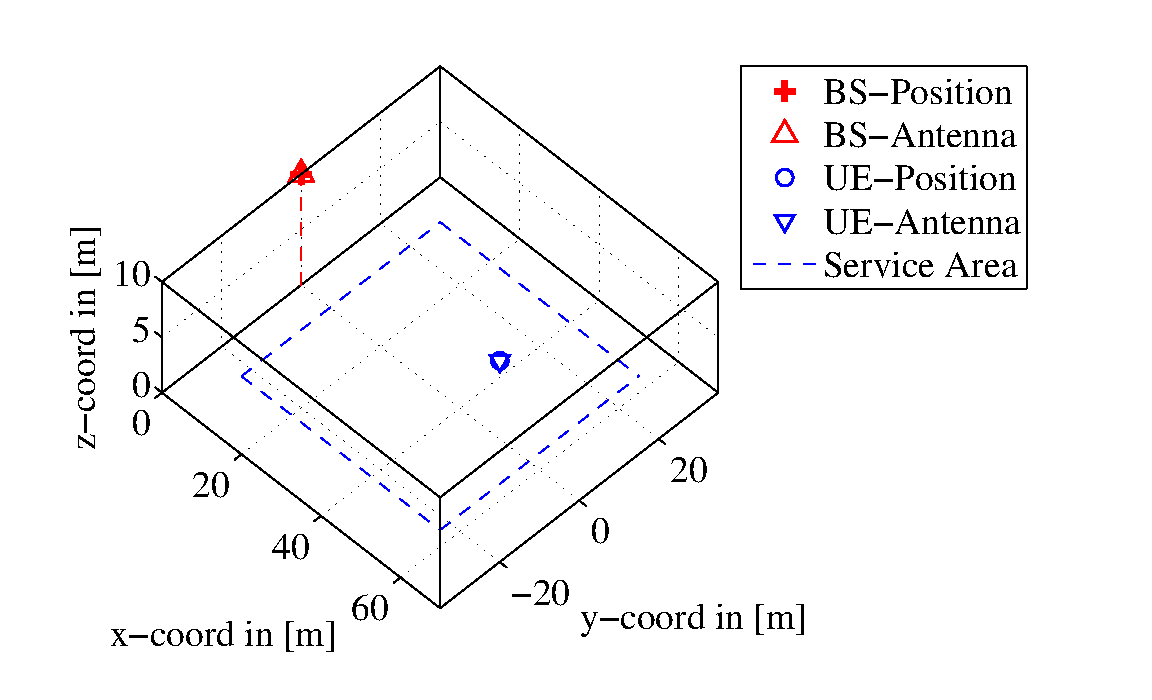
\includegraphics[width=8cm]{Layout_pic_V2.eps}
	\caption{The network layout of the scenario}
	\label{fig:Scenario}
	\vspace{-5mm}
\end{figure}



%\subsection{Experiment Setting}

\subsection{Evaluation of the average signal strength prediction}
%\nt{MSE of the average received power prediction}
\nt{MSE of predicted received signal strength, for Noise-free case and Noisy case}

\subsection{Beam recommendation for analog beamforming}
\nt{The Beam recommendation example}


%\subsection{Experiment XX}
%\nt{spectral efficiency evaluation}

\subsection{Sensing matrix recommendation for hybrid precoder}
%\nt{the sensing matrix recommendation example}
\nt{The sensing matrix recommendation example}

\subsection{Time-varying channel}
\nt{Example for time-varying channel, the propagation environment changes due to mobility.}

\subsection{Online learning}
\nt{Example for online learning.}


\section{Conclusions}








\appendices

\ifCLASSOPTIONcaptionsoff
  \newpage
\fi

\bibliographystyle{IEEEtran}
\bibliography{IEEEabrv,reference} 



\end{document}